\documentclass[11pt]{ainotes}

\title{Machine Learning and Data Mining}
\date{2023 -- 2024}
\def\lastupdate{{PLACEHOLDER-LAST-UPDATE}}

\DeclareAcronym{oltp}{short=OLTP, long=Online Transaction Processing}
\DeclareAcronym{erp}{short=ERP, long=Enterprise Resource Planning}
\DeclareAcronym{mis}{short=MIS, long=Management Information System}
\DeclareAcronym{dss}{short=DSS, long=Decision Support System}
\DeclareAcronym{eis}{short=EIS, long=Executive Information System}
\DeclareAcronym{olap}{short=OLAP, long=Online Analysical Processing}
\DeclareAcronym{bi}{short=BI, long=Business Intelligence}
\DeclareAcronym{dwh}{short=DWH, long=Data Warehouse}
\DeclareAcronym{dm}{short=DM, long=Data Mart}
\DeclareAcronym{etl}{short=ETL, long=Extraction{,} Transformation{,} Loading}
\DeclareAcronym{dfm}{short=DFM, long=Dimensional Fact Model}
\DeclareAcronym{cdc}{short=CDC, long=Change Data Capture}
\DeclareAcronym{crisp}{short=CRISP-DM, long=Cross Industry Standard Process for Data Mining}


\begin{document}

    \makenotesfront
    \printacronyms
    \newpage

    \lohead{\color{gray} Not required for the exam}
\lehead{\color{gray} Not required for the exam}
\chapter{Introduction}


\section{AI systems classification}

\subsection{Intelligence classification}
Intelligence is defined as the ability to perceive or infer information and to retain the knowledge for future use.

\begin{description}
    \item[Weak AI] \marginnote{Weak AI}
        aims to build a system that acts as an intelligent system. 
    
        \item[Strong AI] \marginnote{Strong AI}
        aims to build a system that is actually intelligent. 
\end{description}


\subsection{Capability classification}
\begin{description}
    \item[General AI] \marginnote{General AI}
        systems able to solve any generalized task. 
    
        \item[Narrow AI] \marginnote{Narrow AI}
        systems able to solve a particular task. 
\end{description}


\subsection{AI approaches}
\begin{description}
    \item[Symbolic AI (top-down)] \marginnote{Symbolic AI}
        Symbolic representation of knowledge, understandable by humans.

    \item[Connectionist approach (bottom-up)] \marginnote{Connectionist approach}
        Neural networks. Knowledge is encoded and not understandable by humans.
\end{description}



\section{Symbolic AI}
\begin{description}
    \item[Deductive reasoning] \marginnote{Deductive reasoning}
        Conclude something given some premises (general to specific). 
        It is unable to produce new knowledge.
        \begin{example}
            "All men are mortal" and "Socrates is a man" $\rightarrow$ "Socrates is mortal"
        \end{example}
    
    \item[Inductive reasoning] \marginnote{Inductive reasoning}
        A conclusion is derived from an observation (specific to general).
        Produces new knowledge, but correctness is not guaranteed.
        \begin{example}
            "Several birds fly" $\rightarrow$ "All birds fly"
        \end{example}

    \item[Abduction reasoning] \marginnote{Abduction reasoning}
        An explanation of the conclusion is found from known premises.
        Differently from inductive reasoning, it does not search for a general rule.
        Produces new knowledge, but correctness is not guaranteed.
        \begin{example}
            "Socrates is dead" (conclusion) and "All men are mortal" (knowledge) $\rightarrow$ "Socrates is a man"
        \end{example}
    
    \item[Reasoning by analogy] \marginnote{Reasoning by analogy}
        Principle of similarity (e.g. k-nearest-neighbor algorithm).
        \begin{example}
            "Socrates loves philosophy" and Socrates resembles John $\rightarrow$ "John loves philosophy"
        \end{example}

    \item[Constraint reasoning and optimization] \marginnote{Constraint reasoning}
        Constraints, probability, statistics.
\end{description}


\section{Machine learning}

\subsection{Training approach}
\begin{description}
    \item[Supervised learning] \marginnote{Supervised learning}
        Trained on labeled data (ground truth is known).\\
        Suitable for classification and regression tasks.

    \item[Unsupervised learning] \marginnote{Unsupervised learning}
        Trained on unlabeled data (the system makes its own discoveries).\\
        Suitable for clustering and data mining.

    \item[Semi-supervised learning] \marginnote{Semi-supervised learning}
        The system is first trained to synthesize data in an unsupervised manner,
        followed by a supervised phase.

    \item[Reinforcement learning] \marginnote{Reinforcement learning}
        An agent learns by simulating actions in an environment with rewards and punishments depending on its choices.
\end{description}


\subsection{Tasks}
\begin{description}
    \item[Classification] \marginnote{Classification}
        Supervised task that, given the input variables $X$ and the output (discrete) categories $Y$,
        aims to approximate a mapping function $f: X \rightarrow Y$.

    \item[Regression] \marginnote{Regression}
        Supervised task that, given the input variables $X$ and the output (continuous) variables $Y$,
        aims to approximate a mapping function $f: X \rightarrow Y$.

    \item[Clustering] \marginnote{Clustering}
        Unsupervised task that aims to organize objects into groups.
\end{description}


\subsection{Neural networks}
\marginnote{Perceptron}
A neuron (\textbf{perceptron}) computes a weighted sum of its inputs and 
passes the result to an activation function to produce the output.
\begin{figure}[h]
    \centering
    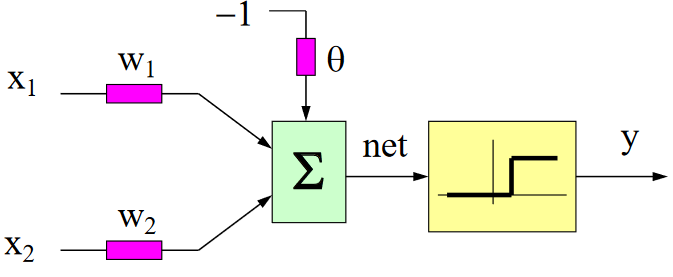
\includegraphics[width=0.40\textwidth]{img/neuron.png}
    \caption{Representation of an artificial neuron}
\end{figure}

\marginnote{Feed-forward neural network}
A \textbf{feed-forward neural network} is composed of multiple layers of neurons, each connected to the next one.
The first layer is the input layer, while the last is the output layer.
Intermediate layers are hidden layers.

The expressivity of a neural network increases when more neurons are used:
\begin{descriptionlist}
    \item[Single perceptron] 
        Able to compute a linear separation.
        \begin{figure}[h]
            \centering
            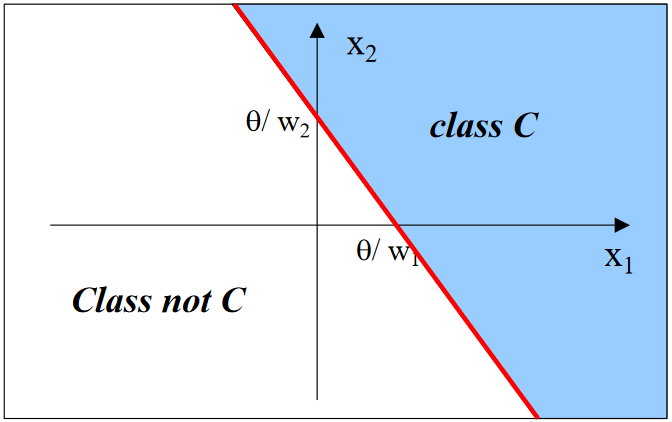
\includegraphics[width=0.25\textwidth]{img/1perceptron.png}
            \caption{Separation performed by one perceptron}
        \end{figure}
    \item[Three-layer network] 
        Able to separate a convex region ($n_\text{edges} \leq n_\text{hidden neurons}$)
        \begin{figure}[h]
            \centering
            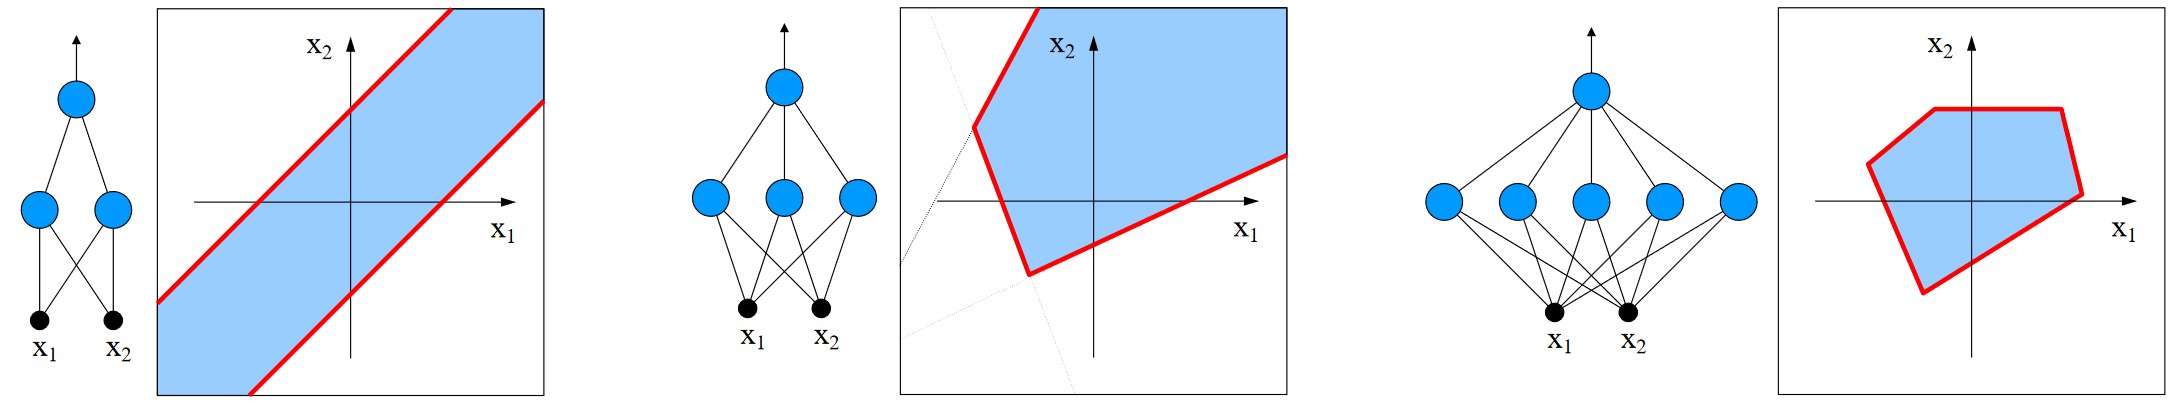
\includegraphics[width=0.90\textwidth]{img/3layer.png}
            \caption{Separation performed by a three-layer network}
        \end{figure}
    \item[Four-layer network] 
        Able to separate regions of arbitrary shape.
        \begin{figure}[h]
            \centering
            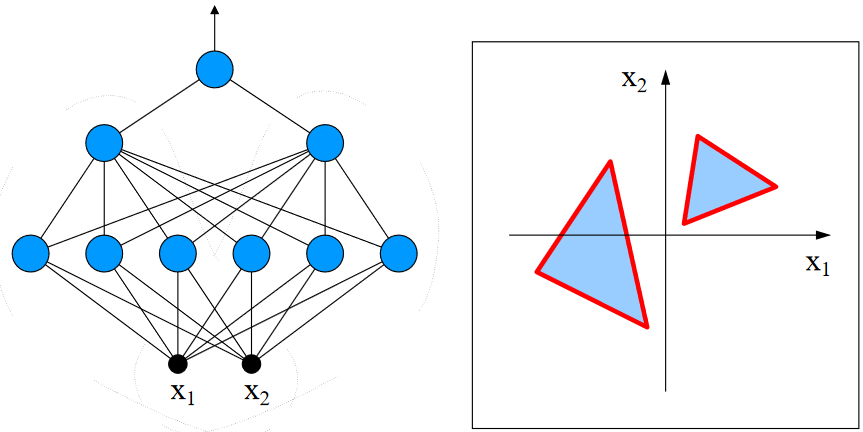
\includegraphics[width=0.40\textwidth]{img/4layer.png}
            \caption{Separation performed by a four-layer network}
        \end{figure}
\end{descriptionlist}

\begin{theorem}[Universal approximation theorem] \marginnote{Universal approximation theorem}
    A feed-forward network with one hidden layer and a finite number of neurons is
    able to approximate any continuous function with desired accuracy.
\end{theorem}

\begin{description}
    \item[Deep learning] \marginnote{Deep learning}
        Neural network with a large number of layers and neurons.
        The learning process is hierarchical: the network exploits simple features in the first layers and
        synthesizes more complex concepts while advancing through the layers.
\end{description}



\section{Automated planning}
Given an initial state, a set of actions and a goal, 
\textbf{automated planning} aims to find a partially or totally ordered sequence of actions to achieve a goal. \marginnote{Automated planning}

An \textbf{automated planner} is an agent that operates in a given domain described by:
\begin{itemize}
    \item Representation of the initial state
    \item Representation of a goal
    \item Formal description of the possible actions (preconditions and effects)
\end{itemize}



\section{Swarm intelligence}
\marginnote{Swarm intelligence}
Decentralized and self-organized systems that result in emergent behaviors. 



\section{Decision support systems}

\begin{description}
    \item[Knowledge based system] \marginnote{Knowledge based system}
        Use knowledge (and data) to support human decisions.
        Bottlenecked by knowledge acquisition.
\end{description}

Different levels of decision support exist:
\begin{descriptionlist}
    \item[Descriptive analytics] \marginnote{Descriptive analytics}
        Data are used to describe the system (e.g. dashboards, reports, \dots).
        Human intervention is required.
            
    \item[Diagnostic analytics] \marginnote{Diagnostic analytics}
        Data are used to understand causes (e.g. fault diagnosis)
        Decisions are made by humans.

    \item[Predictive analytics] \marginnote{Predictive analytics}
        Data are used to predict future evolutions of the system.
        Uses machine learning models or simulators (digital twins)

    \item[Prescriptive analytics] \marginnote{Prescriptive analytics}
        Make decisions by finding the preferred scenario.
        Uses optimization systems, combinatorial solvers or logical solvers.
\end{descriptionlist}


\newpage
\lohead{}
\lehead{}

    \chapter{Data warehouse}


\begin{description}
    \item[\Acl{bi}] \marginnote{\Acl{bi}}
        Transform raw data into information.
        Deliver the right information to the right people at the right time through the right channel.

    \item[\Ac{dwh}] \marginnote{\Acl{dwh}}
        Optimized repository that stores information for decision-making processes.
        \Acp{dwh} are a specific type of \ac{dss}.

        Features:
        \begin{itemize}
            \item Subject-oriented: focused on enterprise-specific concepts.
            \item Integrates data from different sources and provides a unified view.
            \item Non-volatile storage with change tracking. 
        \end{itemize}

    \item[\Ac{dm}] \marginnote{\Acl{dm}}
        Subset of the primary \ac{dwh} with information relevant to a specific business area.
\end{description}



\section{\Acl{olap} (\Acs{olap})}

\begin{description}
    \item[\ac{olap} analyses] \marginnote{\Acl{olap} (\Acs{olap})}
        Able to interactively navigate the information in a data warehouse.
        Allows to visualize different levels of aggregation.

    \item[\ac{olap} session] 
        Navigation path created by the operations that a user applied.
\end{description}

\begin{figure}[ht]
    \centering
    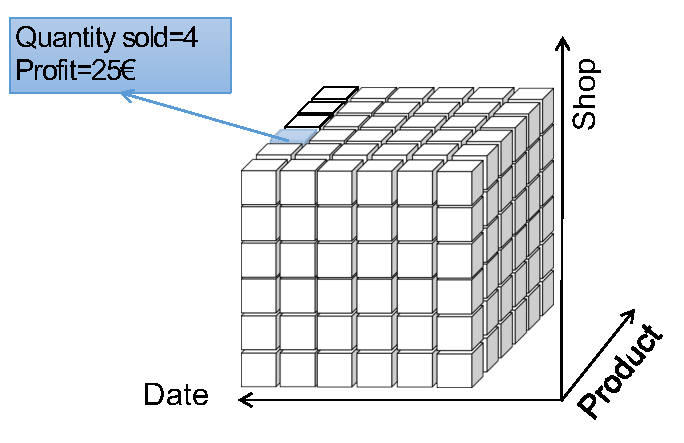
\includegraphics[width=0.35\textwidth]{img/_olap_cube.pdf}
    \caption{\ac{olap} data cube}
\end{figure}


\subsection{Operators}

\begin{description}
    \item[Roll-up] \marginnote{Roll-up}
        \begin{minipage}{0.7\textwidth}
            Increases the level of aggregation (i.e. \texttt{GROUP BY} in SQL).
            Some details are collapsed together.
        \end{minipage}
        \hfill
        \begin{minipage}{0.15\textwidth}
            \centering
            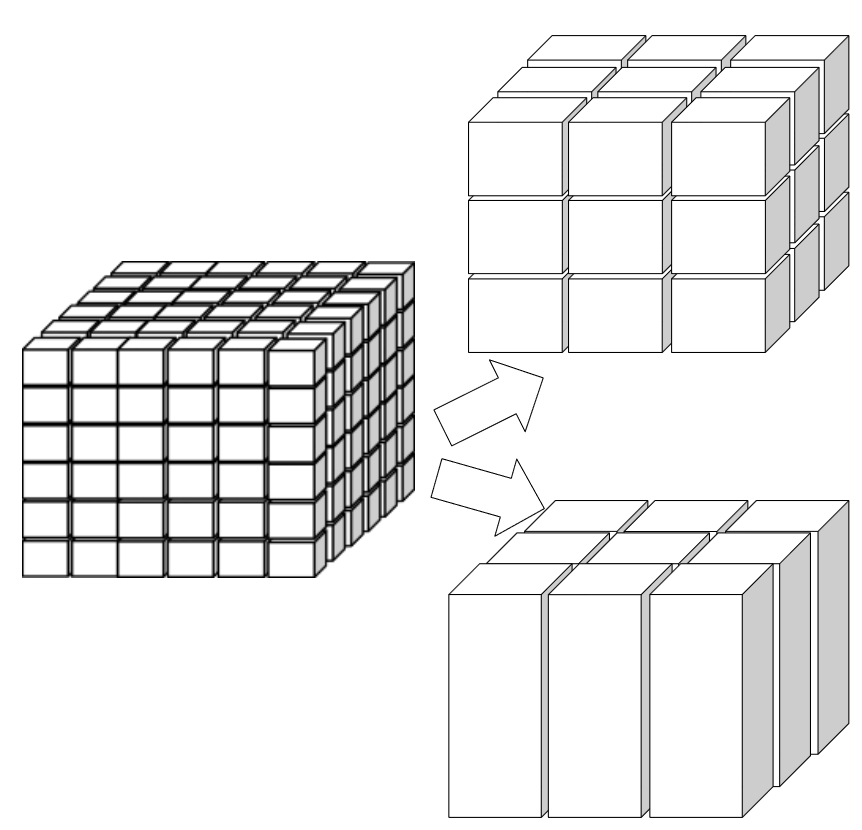
\includegraphics[width=\linewidth]{img/olap_rollup.png}
        \end{minipage}

    \item[Drill-down] \marginnote{Drill-down}
        \begin{minipage}{0.7\textwidth}
            Reduces the level of aggregation.
            Some details are reintroduced.
        \end{minipage}
        \hfill
        \begin{minipage}{0.15\textwidth}
            \centering
            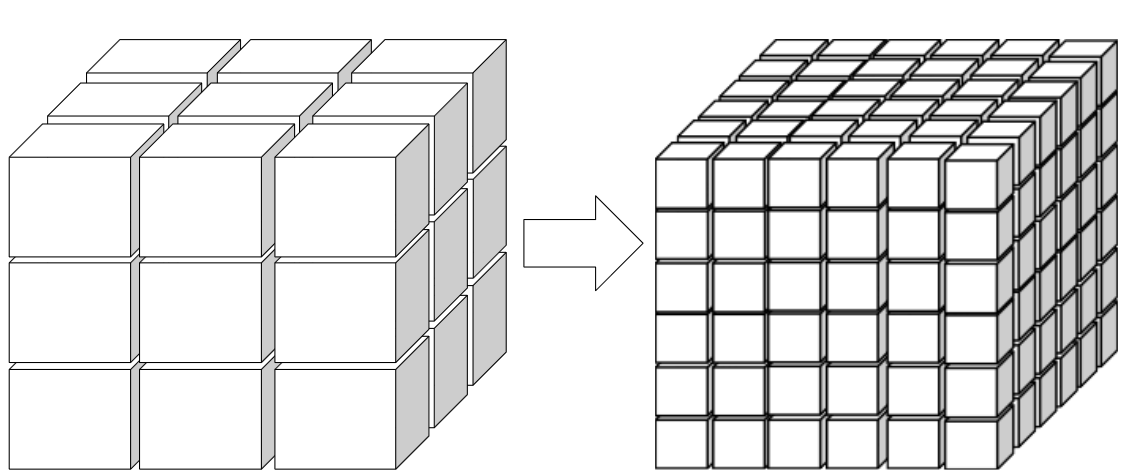
\includegraphics[width=\linewidth]{img/olap_drilldown.png}
        \end{minipage}
    
    \item[Slide-and-dice] \marginnote{Slide-and-dice}
        \begin{minipage}{0.65\textwidth}
            The slice operator reduces the number of dimensions (i.e. drops columns).

            The dice operator reduces the number of data being analyzed (i.e. \texttt{LIMIT} in SQL).
        \end{minipage}
        \hfill
        \begin{minipage}{0.15\textwidth}
            \centering
            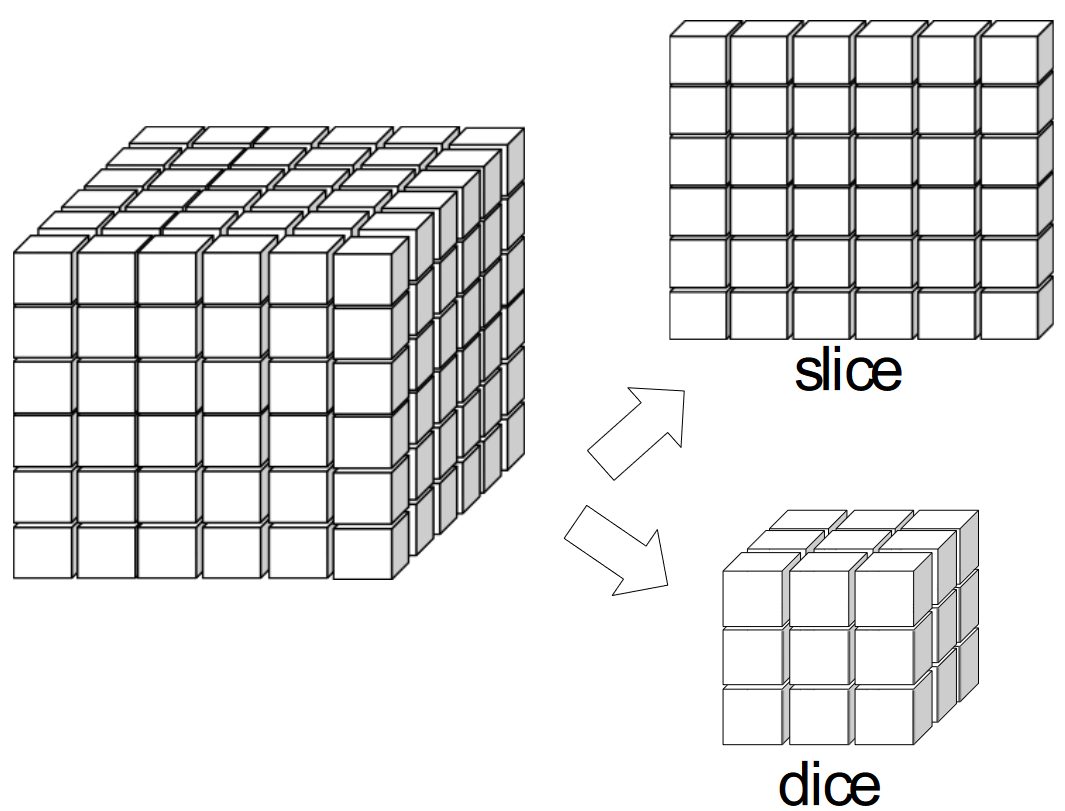
\includegraphics[width=\linewidth]{img/olap_slicedice.png}
        \end{minipage}    

    \item[Pivot] \marginnote{Pivot}
        \begin{minipage}{0.7\textwidth}
            Changes the layout of the data, to analyze it from a different viewpoint.
        \end{minipage}
        \hfill
        \begin{minipage}{0.15\textwidth}
            \centering
            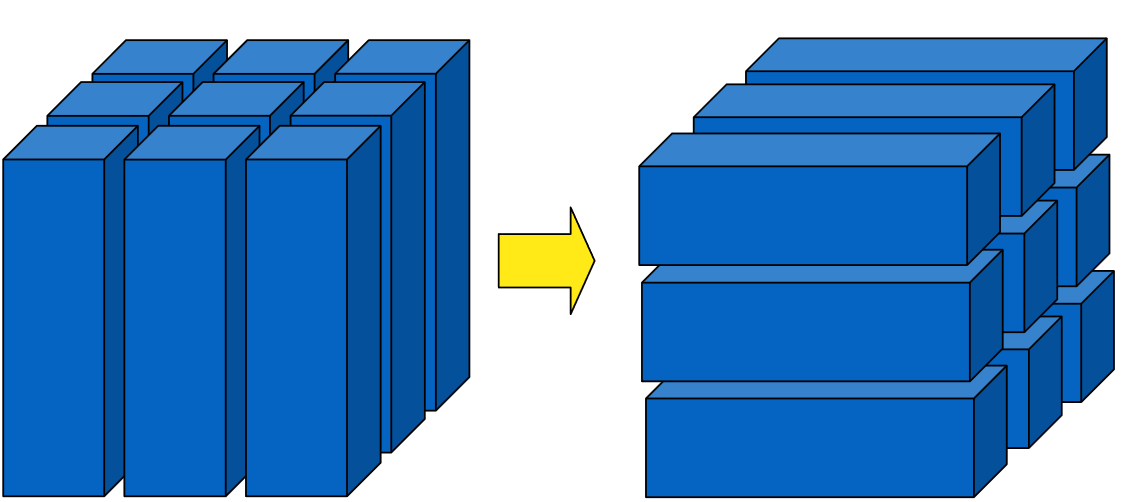
\includegraphics[width=\linewidth]{img/olap_pivot.png}
        \end{minipage}

    \item[Drill-across] \marginnote{Drill-across}
        \begin{minipage}{0.7\textwidth}
            Links concepts from different data sources (i.e. \texttt{JOIN} in SQL).
        \end{minipage}
        \hfill
        \begin{minipage}{0.15\textwidth}
            \centering
            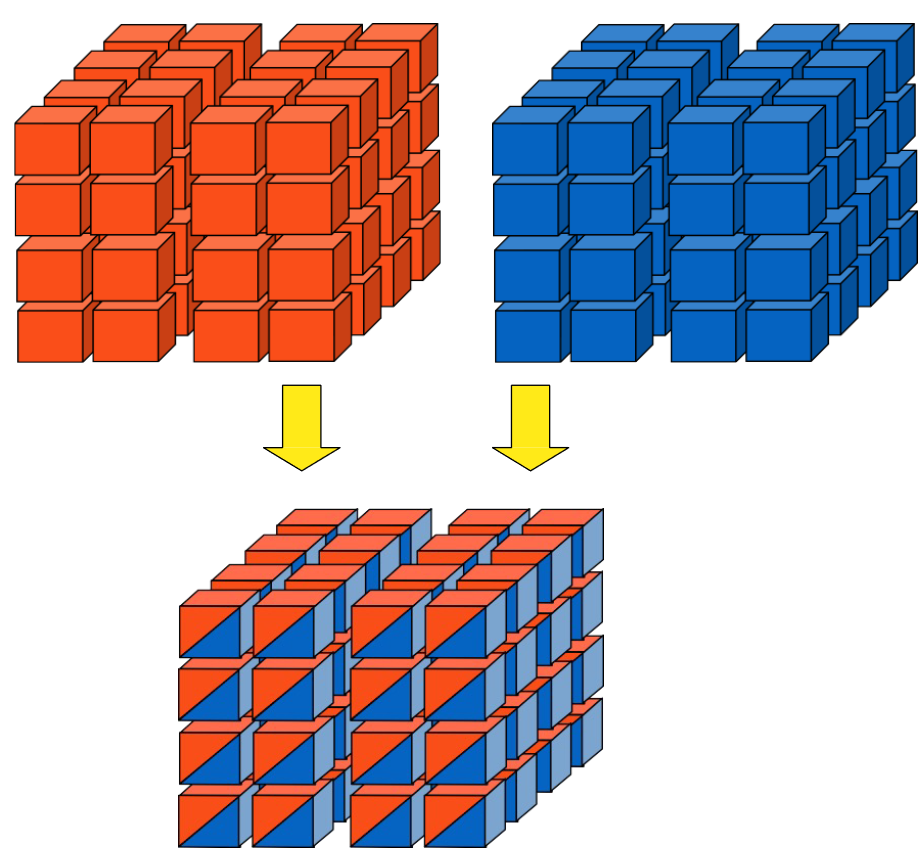
\includegraphics[width=\linewidth]{img/olap_drillacross.png}
        \end{minipage}    
    
    \item[Drill-through] \marginnote{Drill-through}
        Switches from multidimensional aggregated data to operational data (e.g. a spreadsheet).
        \begin{center}
            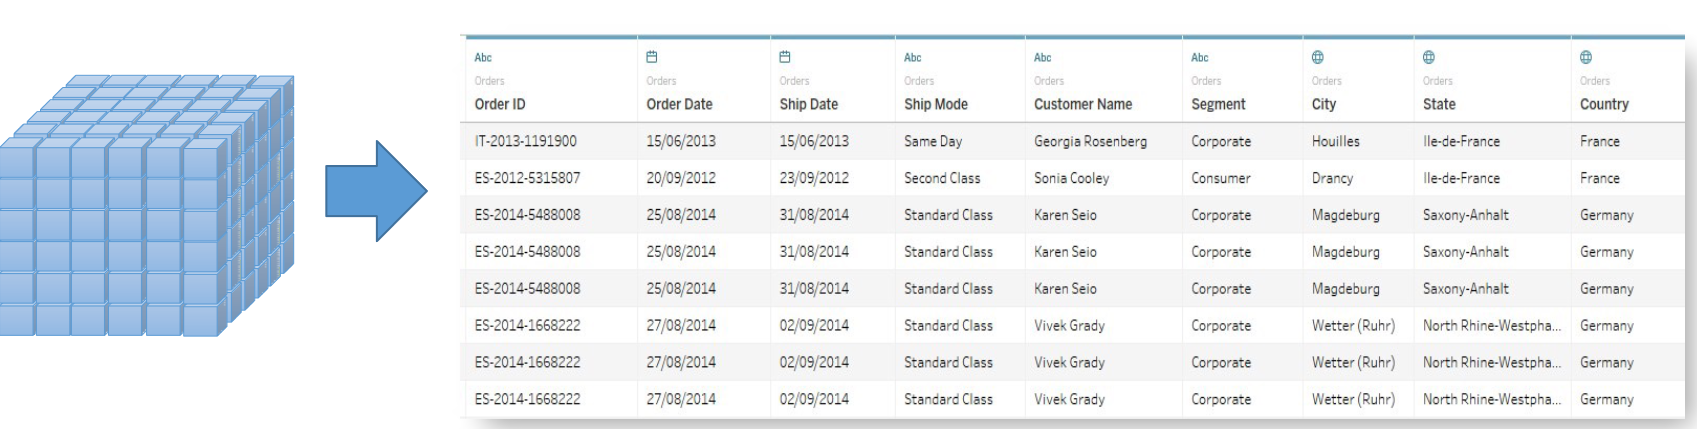
\includegraphics[width=0.5\textwidth]{img/olap_drillthrough.png}
        \end{center}    
\end{description}



\section{\Acl{etl} (\Acs{etl})}
\marginnote{\Acl{etl} (\Acs{etl})}
The \Ac{etl} process extracts, integrates and cleans operational data that will be loaded into a data warehouse.


\subsection{Extraction}

Extracted operational data can be:
\begin{descriptionlist}
    \item[Structured] \marginnote{Strucured data}
        with a predefined data model (e.g. relational DB, CSV)

    \item[Untructured] \marginnote{Unstrucured data}
        without a predefined data model (e.g. social media content)
\end{descriptionlist}

Extraction can be of two types:
\begin{descriptionlist}
    \item[Static] \marginnote{Static extraction}
        The entirety of the operational data are extracted to populate the
        data warehouse for the first time.
    
    \item[Incremental] \marginnote{Incremental extraction}
        Only changes applied since the last extraction are considered.
        Can be based on a timestamp or a trigger.
\end{descriptionlist}


\subsection{Cleaning}

Operational data may contain:
\begin{descriptionlist}
    \item[Duplicate data] 
    \item[Missing data] 
    \item[Improper use of fields] (e.g. saving the phone number in the \texttt{notes} field)
    \item[Wrong values] (e.g. 30th of February)
    \item[Inconsistencies] (e.g. use of different abbreviations)
    \item[Typos]    
\end{descriptionlist}

Methods to clean and increase the quality of the data are:
\begin{descriptionlist}
    \item[Dictionary-based techniques] \marginnote{Dictionary-based cleaning}
        Lookup tables to substitute abbreviations, synonyms or typos.
        Applicable if the domain is known and limited.
        
    \item[Approximate merging] \marginnote{Approximate merging}
        Methods to merge data that do not have a common key.
        \begin{description}
            \item[Approximate join]
                Use non-key attributes to join two tables (e.g. using the name and surname instead of a unique identifier).

            \item[Similarity approach]
                Use similarity functions (e.g. edit distance) to merge multiple instances of the same information
                (e.g. typo in customer surname).
        \end{description}
    
    \item[Ad-hoc algorithms] \marginnote{Ad-hoc algorithms}
\end{descriptionlist}


\subsection{Transformation}
Data are transformed to respect the format of the data warehouse:
\begin{descriptionlist}
    \item[Conversion] \marginnote{Conversion}
        Modifications of types and formats (e.g. date format)
    
    \item[Enrichment] \marginnote{Enrichment}
        Creating new information by using existing attributes (e.g. compute profit from receipts and expenses)

    \item[Separation and concatenation] \marginnote{Separation and concatenation}
        Denormalization of the data: introduces redundancies (i.e. breaks normal form\footnote{\url{https://en.wikipedia.org/wiki/Database_normalization}}) 
        to speed up operations.
\end{descriptionlist}


\subsection{Loading}
Adding data into a data warehouse:
\begin{descriptionlist}
    \item[Refresh] \marginnote{Refresh loading}
        The entire \ac{dwh} is rewritten.

    \item[Update] \marginnote{Update loading}
        Only the changes are added to the \ac{dwh}. Old data are not modified.
\end{descriptionlist}



\section{Data warehouse architectures}

The architecture of a data warehouse should meet the following requirements:
\begin{descriptionlist}
    \item[Separation] Separate the analytical and transactional workflows.
    \item[Scalability] Hardware and software should be easily upgradable.
    \item[Extensibility] Capability to host new applications and technologies without the need to redesign the system.
    \item[Security] Access control.
    \item[Administrability] Easily manageable.
\end{descriptionlist}

\subsection{Single-layer architecture}
\marginnote{Single-layer architecture}
\begin{minipage}{0.55\textwidth}
    \begin{itemize}
        \item Minimizes the amount of data stored (i.e. no redundances).
        \item The source layer is the only physical layer (i.e. no separation).
        \item A middleware provides the \ac{dwh} features.
    \end{itemize}
\end{minipage}
\hfill
\begin{minipage}{0.4\textwidth}
    \centering
    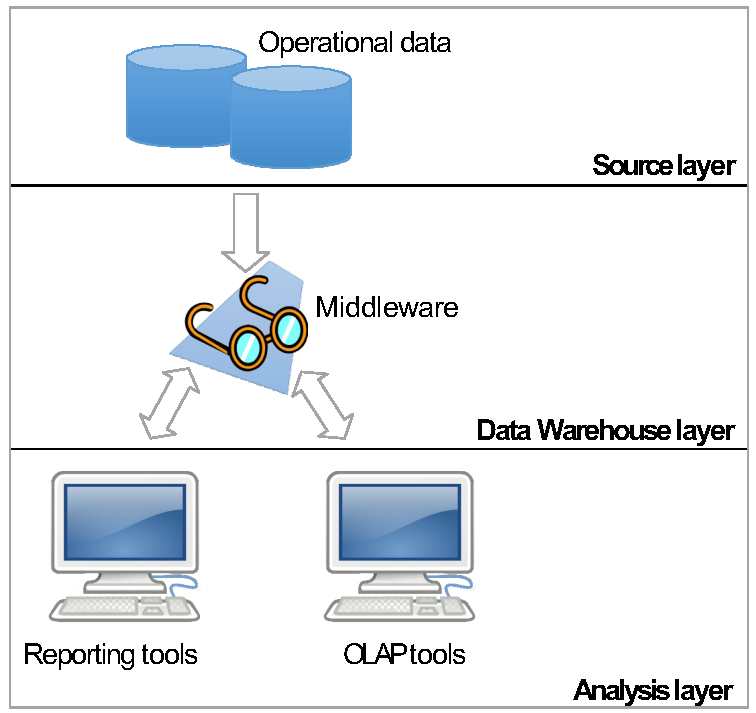
\includegraphics[width=\linewidth]{img/_1layer_dwh.pdf}
\end{minipage}


\subsection{Two-layer architecture}
\marginnote{Two-layer architecture}
\begin{minipage}{0.55\textwidth}
    \begin{itemize}
        \item Source data (source layer) are physically separated from the \ac{dwh} (data warehouse layer).
        \item A staging layer applies \ac{etl} procedures before populating the \ac{dwh}.
        \item The \ac{dwh} is a centralized repository from which data marts can be created.
            Metadata repositories store information on sources, staging and data marts schematics.
    \end{itemize}
\end{minipage}
\hfill
\begin{minipage}{0.4\textwidth}
    \centering
    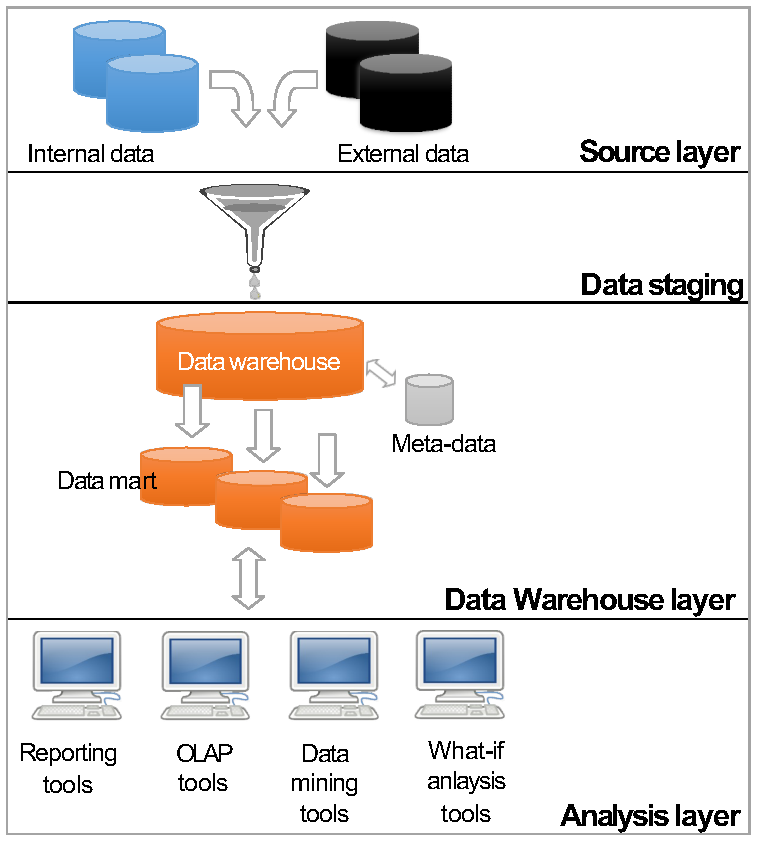
\includegraphics[width=\linewidth]{img/_2layer_dwh.pdf}
\end{minipage}


\subsection{Three-layer architecture}
\marginnote{Three-layer architecture}
\begin{minipage}{0.45\textwidth}
    \begin{itemize}
        \item A reconciled layer enhances the cleaned data coming from the staging step by 
            adding enterprise-level details (i.e. adds more redundancy before populating the \ac{dwh}).
    \end{itemize}
\end{minipage}
\hfill
\begin{minipage}{0.5\textwidth}
    \centering
    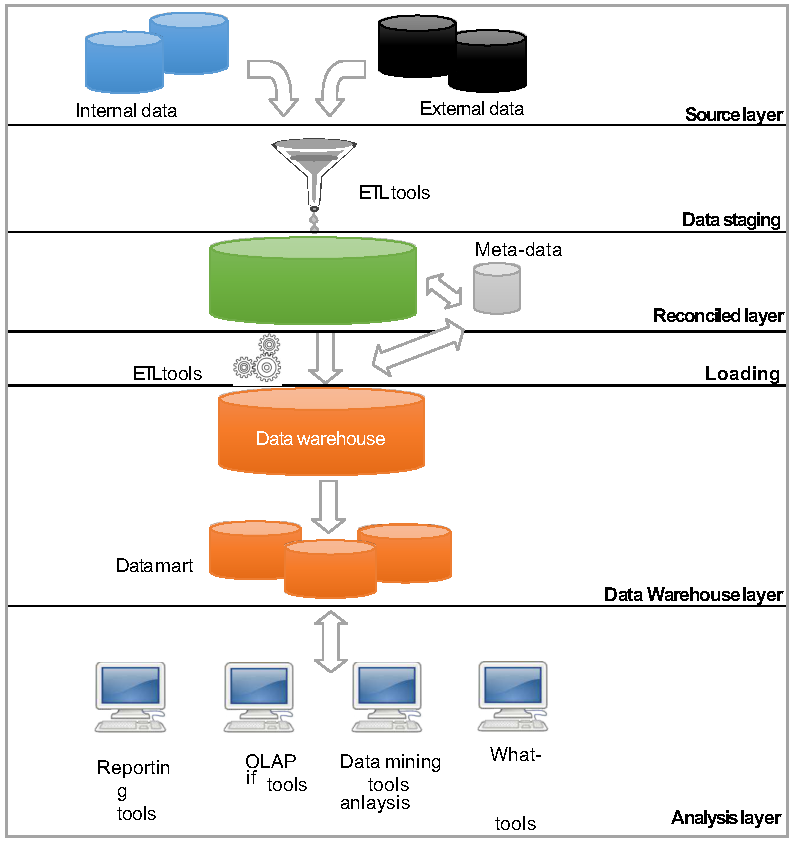
\includegraphics[width=\linewidth]{img/_3layer_dwh.pdf}
\end{minipage}



\section{Conceptual modeling}

\begin{description}
    \item[\Acl{dfm} (\acs{dfm})] \marginnote{\Acl{dfm} (\acs{dfm})}
        Conceptual model to support the design of data marts.
        The main concepts are:
        \begin{descriptionlist}
            \item[Fact] 
                Concept relevant to decision-making processes (e.g. sales).
            \item[Measure]
                Numerical property to describe a fact (e.g. profit).
            \item[Dimension] 
                Property of a fact with a finite domain (e.g. date).
            \item[Dimensional attribute] 
                Property of a dimension (e.g. month).
            \item[Hierarchy] 
                A tree where the root is a dimension and nodes are dimensional attributes (e.g. date $\rightarrow$ month).
            \item[Primary event] 
                Occurrence of a fact. It is described by a tuple with a value for each dimension and each measure.
            \item[Secondary event] 
                Aggregation of primary events. 
                Measures of primary events are aggregated if they have the same (preselected) dimensional attributes.
        \end{descriptionlist}
\end{description}

\begin{figure}[ht]
    \centering
    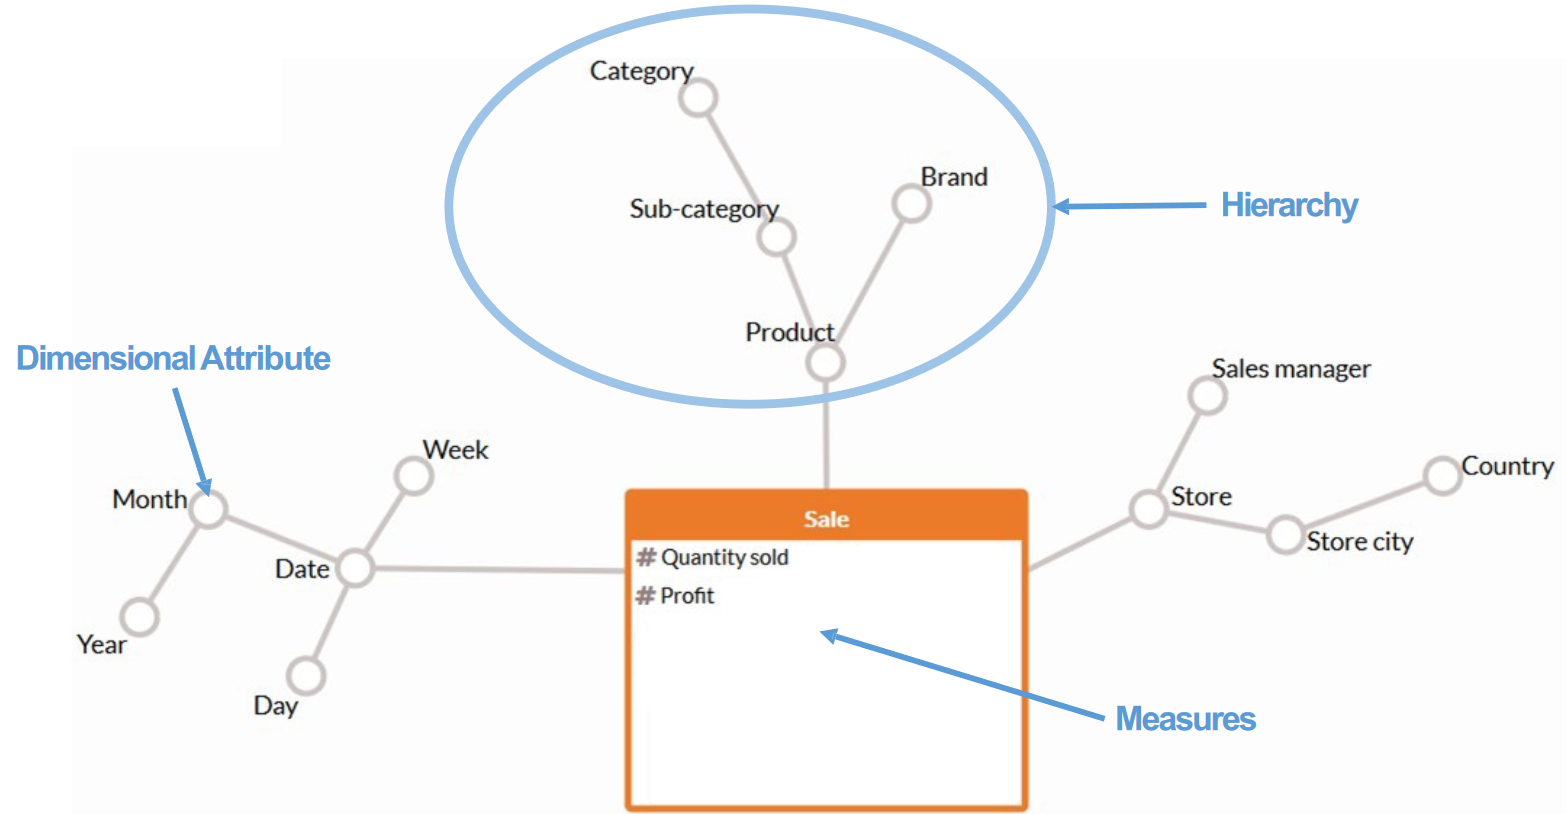
\includegraphics[width=0.8\textwidth]{img/dfm.png}
    \caption{Example of \ac{dfm}}
\end{figure}

\begin{figure}[ht]
    \centering
    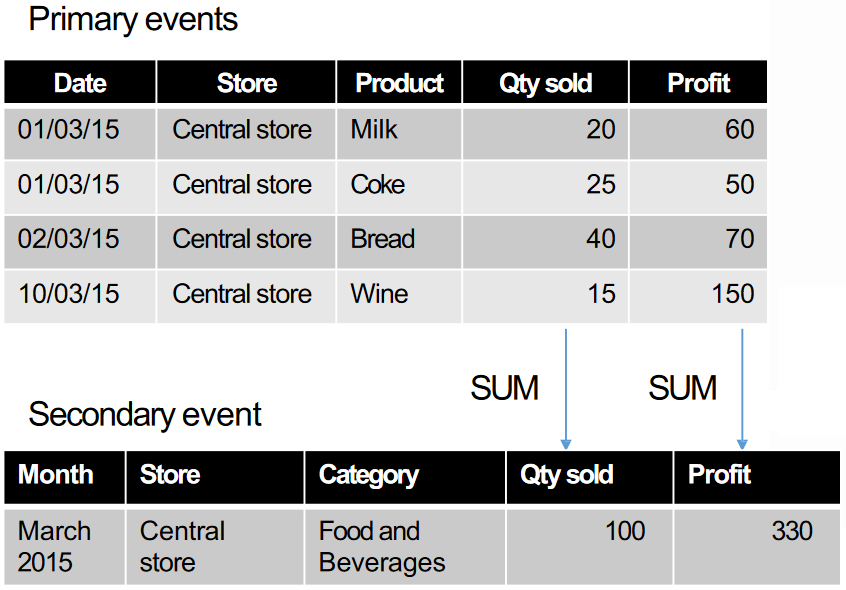
\includegraphics[width=0.5\textwidth]{img/dfm_events.png}
    \caption{Example of primary and secondary events}
\end{figure}


\subsection{Aggregation operators}

Measures can be classified as:
\begin{descriptionlist}
    \item[Flow measures] \marginnote{Flow measures}
        Evaluated cumulatively with respect to a time interval (e.g. quantity sold).
    \item[Level measures] \marginnote{Level measures}
        Evaluated at a particular time (e.g. number of products in inventory).
    \item[Unit measures] \marginnote{Unit measures}
        Evaluated at a particular time but expressed in relative terms (e.g. unit price).
\end{descriptionlist}

Aggregation operators can be classified as:
\begin{descriptionlist}
    \item[Distributive] \marginnote{Distributive operators}
        Able to calculate aggregates from partial aggregates (e.g. \texttt{SUM}, \texttt{MIN}, \texttt{MAX}).
    \item[Algebraic] \marginnote{Algebraic operators}
        Requires a finite number of support measures to compute the result (e.g. \texttt{AVG}).
    \item[Holistic] \marginnote{Holistic operators}
        Requires an infinite number of support measures to compute the result (e.g. \texttt{RANK}).
\end{descriptionlist}

\begin{description}
    \item[Additivity] \marginnote{Additive measure}
    A measure is additive along a dimension if an aggregation operator can be applied. 
    \begin{table}[ht]
        \centering
        \begin{tabular}{l | c | c}
                                        & \textbf{Temporal hierarchies}                             & \textbf{Non-temporal hierarchies} \\
            \hline
            \textbf{Flow measures}      & \texttt{SUM}, \texttt{AVG}, \texttt{MIN}, \texttt{MAX}    & \texttt{SUM}, \texttt{AVG}, \texttt{MIN}, \texttt{MAX} \\
            \textbf{Level measures}     & \texttt{AVG}, \texttt{MIN}, \texttt{MAX}                  & \texttt{SUM}, \texttt{AVG}, \texttt{MIN}, \texttt{MAX} \\
            \textbf{Unit measures}      & \texttt{AVG}, \texttt{MIN}, \texttt{MAX}                  & \texttt{AVG}, \texttt{MIN}, \texttt{MAX} \\
        \end{tabular}
        \caption{Allowed operators for each measure type}
    \end{table}
\end{description}



\section{Logical design}
\marginnote{Logical design}
Defining the data structures (e.g. tables and relationships) according to a conceptual model.
There are two main strategies:
\begin{descriptionlist}
    \item[Star schema] \marginnote{Star schema}
        A fact table that contains all the measures is linked to dimensional tables.
        \begin{figure}[ht]
            \centering
            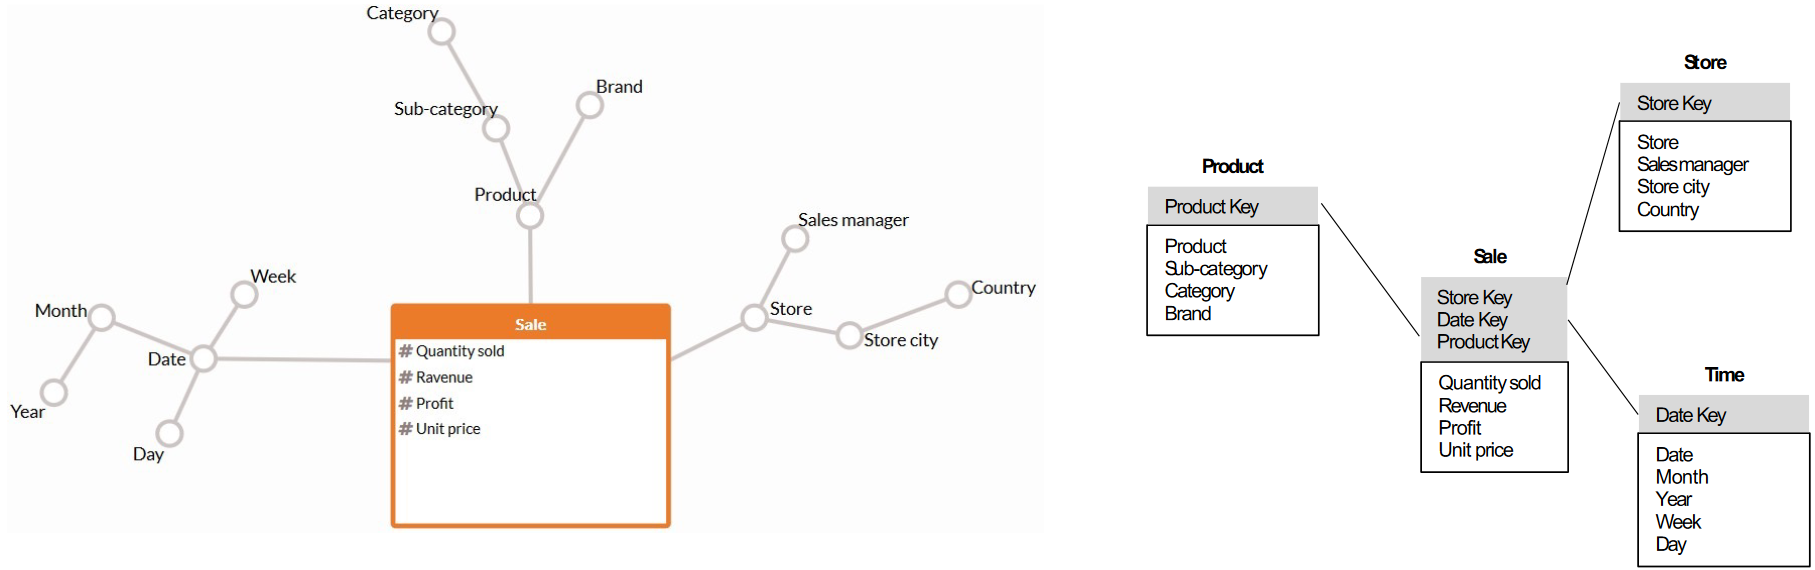
\includegraphics[width=\textwidth]{img/logical_star_schema.png}
            \caption{Example of star schema}
        \end{figure}

    \item[Snowflake schema] \marginnote{Snowflake schema}
        A star schema variant with partially normalized dimensional tables.
        \begin{figure}[H]
            \centering
            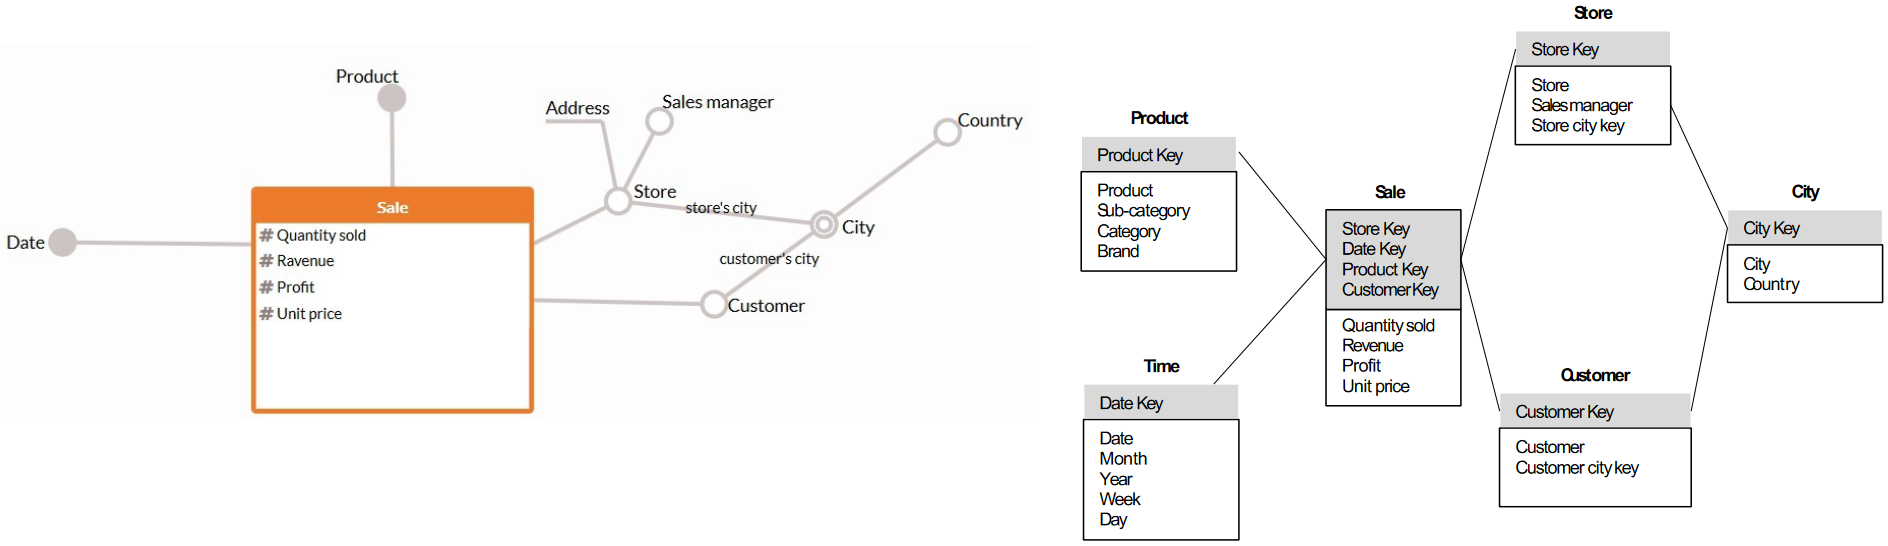
\includegraphics[width=\textwidth]{img/logical_snowflake_schema.png}
            \caption{Example of snowflake schema}
        \end{figure}
\end{descriptionlist}
    \chapter{Data lake}

\begin{description}
    \item[Dark data] \marginnote{Dark data}
        Acquired and stored data that are never used for decision-making processes.

    \item[Data lake] \marginnote{Data lake}
        Repository to store raw (unstructured) data.
        It has the following features:
        \begin{itemize}
            \item Does not enforce a schema on write.
            \item Allows flexible access and applies schemas on read.
            \item Single source of truth.
            \item Low cost and scalable.
        \end{itemize}

    \item[Storage]
        Stored data can be classified as:
        \begin{descriptionlist}
            \item[Hot] \marginnote{Hot storage}
                A low volume of highly requested data that require low latency.
                More expensive HW/SW.
            \item[Cold] \marginnote{Cold storage}
                A large amount of data that does not have latency requirements.
                Less expensive.
        \end{descriptionlist}

        \begin{figure}[ht]
            \centering
            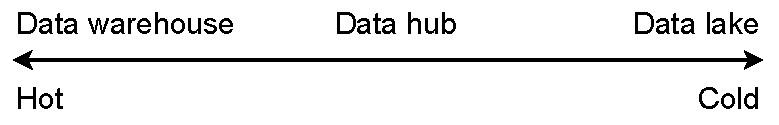
\includegraphics[width=0.5\textwidth]{img/_storage.pdf}
            \caption{Data storage technologies}
        \end{figure}
\end{description}


\section{Traditional vs insight-driven data systems}
\begin{tabular}{c | p{0.4\textwidth} | p{0.4\textwidth}}
    & \textbf{\makecell[c]{Traditional (data warehouse)}} & \textbf{\makecell[c]{Insight-driven (data lake)}} \\
    \hline
    \textbf{Sources} & Structured data & Structured, semi-structured and unstructured data \\
    \hline
    \textbf{Storage} & Limited ingestion and storage capability & Virtually unlimited ingestion and storage capability \\
    \hline
    \textbf{Schema} & Schema designed upfront & Schema not fixed \\
    \hline
    \textbf{Transformations} & \ac{etl} upfront & Transformations on query \\
    \hline
    \textbf{Analytics} & SQL, \ac{bi} tools, full-text search & Traditional methods, self-service \ac{bi}, big data, machine learning, \dots \\
    \hline
    \textbf{Price} & High storage cost & Low storage cost \\
    \textbf{Performance} & Fast queries & Scalability/speed/cost tradeoffs \\
    \hline
    \textbf{Quality} & High data quality & Depends on the use case \\
\end{tabular}


\section{Data architecture evolution}
\begin{description}
    \item[Traditional data warehouse] \marginnote{Traditional data warehouse} 
        (i.e. in-house data warehouse)
        \begin{itemize}
            \item Structured data with predefined schemas.
            \item High setup and maintenance cost. Not scalable.
            \item Relational high-quality data.
            \item Slow data ingestion.
        \end{itemize}

    \item[Modern cloud data warehouse] \marginnote{Modern cloud data warehouse} 
        \phantom{}
        \begin{itemize}
            \item Structured and semi-structured data.
            \item Low setup and maintenance cost. Scalable and easier disaster recovery.
            \item Relational high-quality data and mixed data.
            \item Fast data ingestion if supported.
        \end{itemize}

    \item[On-premise big data] \marginnote{On-premise big data} 
        (i.e. in-house data lake)
        \begin{itemize}
            \item Any type of data with schemas on read.
            \item High setup and maintenance cost.
            \item Fast data ingestion.
        \end{itemize}

    \item[Cloud data lake] \marginnote{Cloud data lake} 
        \phantom{}
        \begin{itemize}
            \item Any type of data with schemas on read.
            \item Low setup and maintenance cost. Scalable and easier disaster recovery.
            \item Fast data ingestion.
        \end{itemize}
\end{description}


\section{Components}

\subsection{Data ingestion} 
\marginnote{Data ingestion}
    \begin{descriptionlist}
        \item[Workload migration]
            Inserting all the data from an existing source.
        \item[Incremental ingestion]
            Inserting changes since the last ingestion.
        \item[Streaming ingestion]   
            Continuously inserting data.
    \end{descriptionlist}

    \begin{description}
        \item[\Acl{cdc} (\Acs{cdc})] \marginnote{\Acl{cdc} (\Acs{cdc})}
            Mechanism to detect changes and insert the new data into the data lake (possibly in real-time).
    \end{description}

\subsection{Storage}
\begin{descriptionlist}
    \item[Raw] \marginnote{Raw storage}
        Immutable data useful for disaster recovery.
    \item[Optimized] \marginnote{Optimized storage}
        Optimized raw data for faster query.
    \item[Analytics] \marginnote{Analytics storage}
        Ready to use data.
\end{descriptionlist}

\begin{description}
    \item[Columnar storage] \phantom{}
        \begin{itemize}
            \item Homogenous data are stores contiguously.
            \item Speeds up methods that process entire columns (i.e. all the values of a feature).
            \item Insertion becomes slower.
        \end{itemize}

    \item[Data catalog]
        Methods to add descriptive metadata to a data lake.
        This is useful to prevent an unorganized data lake (data swamp).
\end{description}
        
\subsection{Processing and analytics} 
\marginnote{Processing and analytics}
\begin{descriptionlist}
    \item[Interactive analytics]
        Interactive queries to large volumes of data.
        The results are stored back in the data lake.
    \item[Big data analytics]
        Data aggregations and transformations.
    \item[Real-time analytics]   
        Streaming analysis.
\end{descriptionlist}


\section{Architectures}

\subsection{Lambda lake} 
\marginnote{Lambda lake}
\begin{description}
    \item[Batch layer] Receives and stores the data. Prepares the batch views for the serving layer.
    \item[Serving layer] Indexes batch views for faster queries.
    \item[Speed layer] Receives the data and prepares real-time views. The views are also stored in the serving layer.
\end{description}
\begin{figure}[ht]
    \centering
    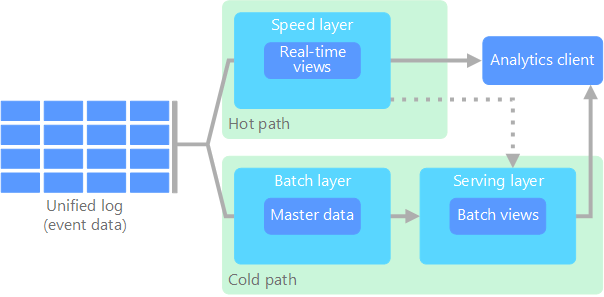
\includegraphics[width=0.5\textwidth]{img/lambda_lake.png}
    \caption{Lambda lake architecture}
\end{figure}

\subsection{Kappa lake} 
\marginnote{Kappa lake}
The data are stored in a long-term store.
Computations only happen in the speed layer (avoids lambda lake redundancy between batch layer and speed layer).
\begin{figure}[ht]
    \centering
    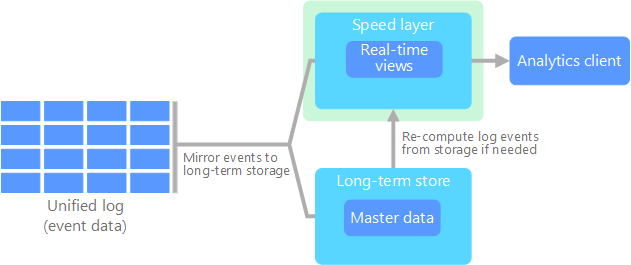
\includegraphics[width=0.5\textwidth]{img/kappa_lake.png}
    \caption{Kappa lake architecture}
\end{figure}

\subsection{Delta lake} 
\marginnote{Delta lake}
Framework that adds features on top of an existing data lake.
\begin{itemize}
    \item ACID transactions
    \item Scalable metadata handling
    \item Data versioning
    \item Unified batch and streaming
    \item Schema enforcement
\end{itemize}
\begin{figure}[ht]
    \centering
    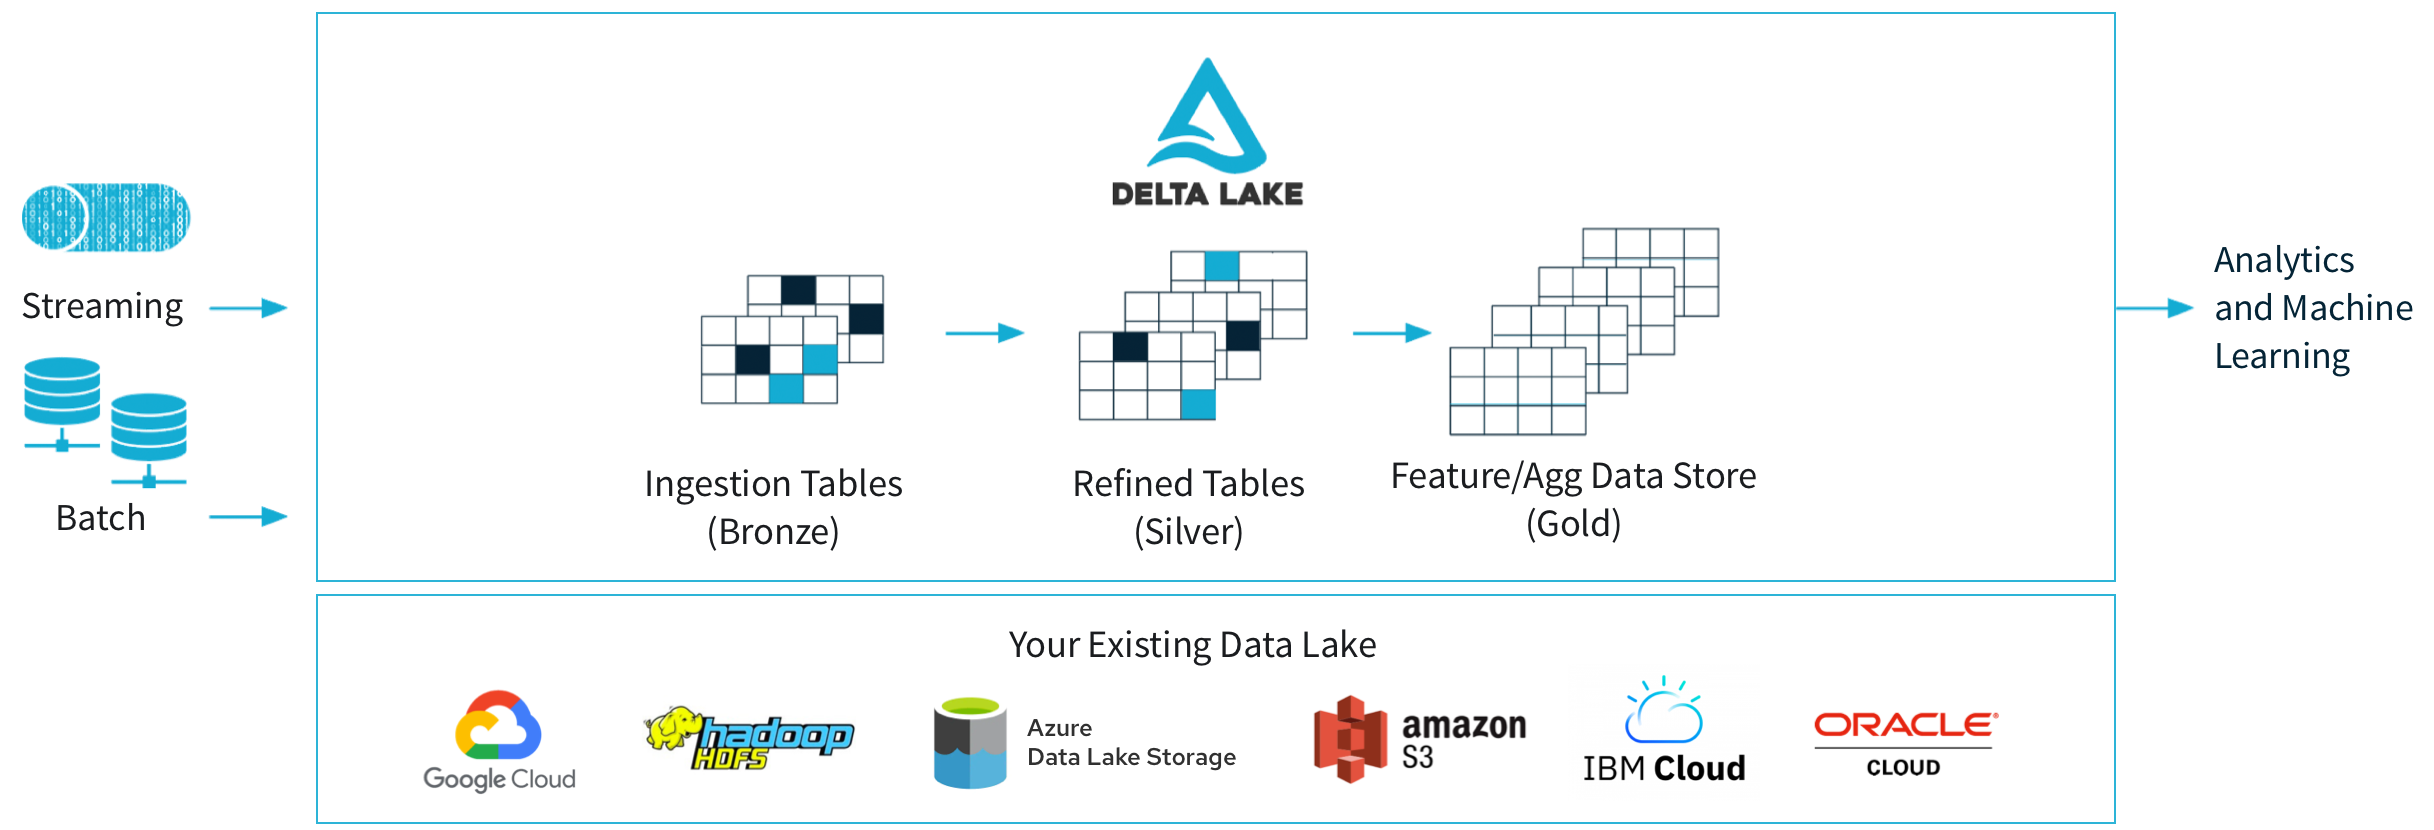
\includegraphics[width=0.7\textwidth]{img/delta_lake.png}
    \caption{Delta lake architecture}
\end{figure}


\section{Metadata}
\marginnote{Metadata}
Metadata are used to organize a data lake.
Useful metadata are:
\begin{descriptionlist}
    \item[Source] Origin of the data.
    \item[Schema] Structure of the data.
    \item[Format] File format or encoding.
    \item[Quality metrics] (e.g. percentage of missing values).
    \item[Lifecycle] Retention policies and archiving rules.
    \item[Ownership] 
    \item[Lineage] History of applied transformations or dependencies.
    \item[Access control] 
    \item[Classification] Sensitivity level of the data.
    \item[Usage information] Record of who accessed the data and how it is used.
\end{descriptionlist}
    \chapter{CRISP-DM}

\begin{description}
    \item[\Acl{crisp}] \marginnote{\acs{crisp}}
        Standardized process for data mining.
        \begin{figure}[ht]
            \centering
            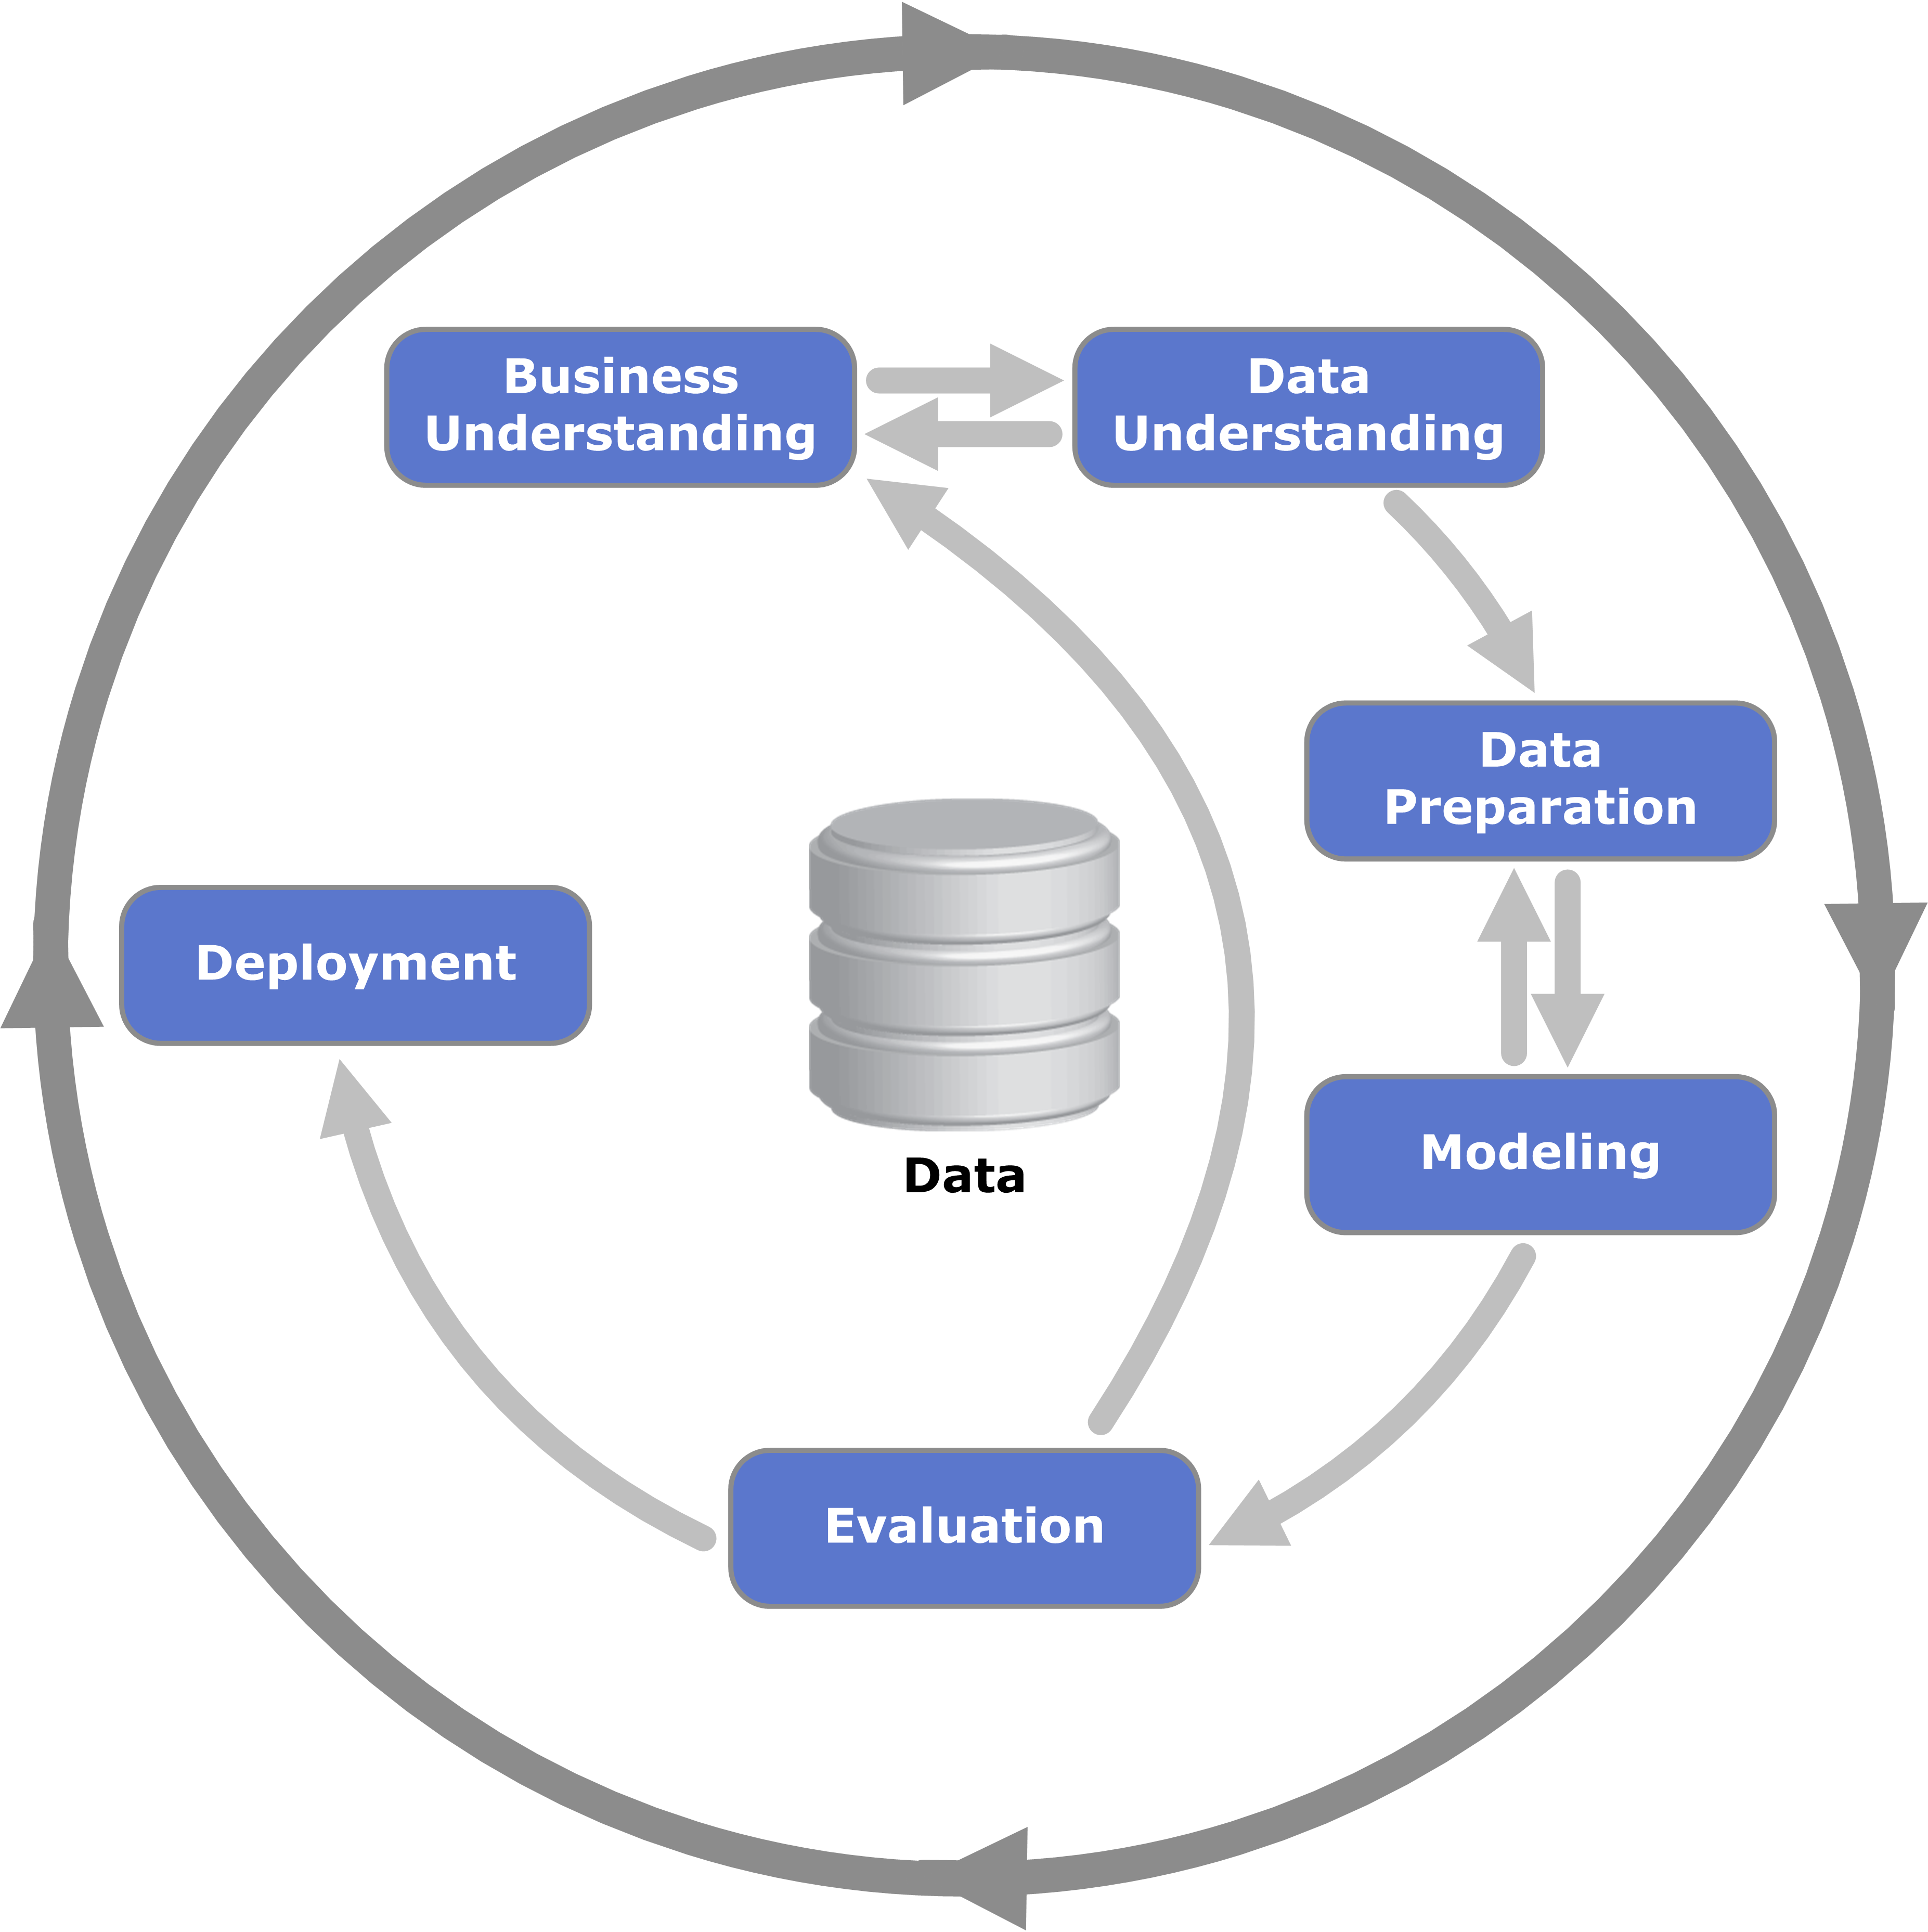
\includegraphics[width=0.45\textwidth]{img/crisp.png}
            \caption{\ac{crisp} workflow}
        \end{figure}
\end{description}


\section{Business understanding}
\begin{itemize}
    \item Determine the objective and the success criteria.
    \marginnote{Business understanding}
    \item Feasibility study.
    \item Produce a plan.
\end{itemize}

\section{Data understanding}
\begin{itemize}
    \item Determine the available (raw) data.
    \marginnote{Data understanding}
    \item Determine the cost of the data.
    \item Collect, describe, explore and verify data.
\end{itemize}

\section{Data preparation}
\begin{itemize}
    \item Data cleaning.
    \marginnote{Data preparation}
    \item Data transformations.
\end{itemize}

\section{Modeling}
\begin{itemize}
    \item Select modeling technique.
    \marginnote{Modeling}
    \item Build/train the model.
\end{itemize}

\section{Evaluation}
\begin{itemize}
    \item Evaluate results.
    \marginnote{Evaluation}
    \item Review process.
\end{itemize}

\section{Deployment}
\begin{itemize}
    \item Plan deployment.
    \marginnote{Deployment}
    \item Plan monitoring and maintenance.
    \item Final report and review.
\end{itemize}

    \chapter{Machine learning}


\section{Models}

\begin{description}
    \item[Function model] \marginnote{Function model}
        The model (predictor) is a deterministic function:
        \[ f: \mathbb{R}^D \rightarrow \mathbb{R} \]

        In this course, only linear functions are considered:
        \[ f_\vec{\uptheta}(\vec{x}) = \uptheta_0 + \uptheta_1 x_1 + \dots + \uptheta_D x_D = \vec{\uptheta}^T \vec{x} \]
        where $\vec{x} = \begin{pmatrix} 1, x_1, \dots, x_D \end{pmatrix}$ is the input vector and
        $\vec{\uptheta} = \begin{pmatrix} \uptheta_0, \dots, \uptheta_D \end{pmatrix}$ is the parameter vector.

    \item[Probabilistic model] \marginnote{Probabilistic model}
        The model is a multivariate probabilistic distribution.
\end{description}



\section{Learning}

\subsection{Empirical risk minimization}
\marginnote{Empirical risk minimization}
Used for function models.

Let $(\vec{x}_n, y_n)$ be a dataset of $N$ elements
where $\vec{x}_n \in \mathbb{R}^D$ are the examples and $y_n \in \mathbb{R}$ are the labels.
We want to estimate a predictor $f_\vec{\uptheta}(\vec{x}) = \vec{\uptheta}^T \vec{x}$ with parameters $\vec{\uptheta}$
such that, with the ideal parameters $\vec{\uptheta}^*$, it fits the data well:
\[ f_{\vec{\uptheta}^*}(\vec{x}_n) \approx y_n \]

We denote the output of the estimator as $\hat{y}_n = f_\vec{\uptheta}(\vec{x}_n)$.

\begin{description}
    \item[Loss function] \marginnote{Loss function}
        A loss function $\ell(y_n, \hat{y}_n)$ indicates how a predictor fits the data.

        An assumption commonly made in machine learning is that 
        the dataset $(\vec{x}_n, y_n)$ is independent and identically distributed. 
        Therefore, the empirical mean is a good estimate of the population mean.

        \begin{description}
            \item[Empirical risk] \marginnote{Empirical risk}
                Given the example matrix $\matr{X} = \begin{pmatrix} \vec{x}_1, \dots, \vec{x}_N \end{pmatrix} \in \mathbb{R}^{N \times D}$
                and the label vector $\vec{y} = \begin{pmatrix} y_1, \dots, y_N \end{pmatrix} \in \mathbb{R}^N$.
                The empirical risk is given by the average loss:
                \[ \textbf{R}_\text{emp}(f_\vec{\uptheta}, \matr{X}, \vec{y}) = \frac{1}{N} \sum_{n=1}^{N} \ell(y_n, \hat{y}_n) \]

            \begin{example}[Least-squares loss] \marginnote{Least-squares loss}
                The least-squares loss is defined as:
                \[ \ell(y_n, \hat{y}_n) = (y_n - \hat{y}_n)^2 \]

                Therefore, the minimization task is:
                \[ 
                    \min_{\vec{\uptheta} \in \mathbb{R}^D} \frac{1}{N} \sum_{n=1}^{N} (y_n - f_\vec{\uptheta}(\vec{x}_n))^2 =
                    \min_{\vec{\uptheta} \in \mathbb{R}^D} \frac{1}{N} \sum_{n=1}^{N} (y_n - \vec{\uptheta}^T\vec{x}_n)^2 =
                    \min_{\vec{\uptheta} \in \mathbb{R}^D} \frac{1}{N} \Vert \vec{y} - \matr{X}\vec{\uptheta} \Vert^2
                \]
            \end{example}

            \item[Expected risk] \marginnote{Expected risk}
                The expected risk is defined as:
                \[ \textbf{R}_\text{true}(f_\vec{\uptheta}) = \mathbb{E}_{\vec{x}, y}[\ell(y, f_\vec{\uptheta}(\vec{x}_\text{test}))] \]
                where the parameters $\vec{\uptheta}$ are fixed and the samples are taken from a test set.

            \item[Overfitting] \marginnote{Overfitting}
                A predictor $f_\vec{\uptheta}$ is overfitting when $\textbf{R}_\text{emp}(f, \matr{X}_\text{train}, \vec{y}_\text{train})$
                underestimates $\textbf{R}_\text{true}(f_\vec{\uptheta})$ (i.e. the loss on the training set is low, but on the test set is high).

            \item[Regularization] \marginnote{Regularization}
                Method that introduces a penalty term to the loss that
                helps to find a compromise between the accuracy and the complexity of the solution:
                \[ \bar{\ell}(y_n, \hat{y}_n) = \ell(y_n, \hat{y}_n) + \lambda \mathcal{R}(\vec{\uptheta}) \]
                where $\lambda \in \mathbb{R}^+$ is the regularization parameter and $\mathcal{R}$ is the penalty.
        \end{description}
\end{description}



\subsection{Maximum likelihood}
\marginnote{Maximum likelihood}
Used for probabilistic models.
    \chapter{Data preprocessing}

\section{Aggregation}
\marginnote{Aggregation}

Combining multiple attributes into a single one.
Useful for:
\begin{descriptionlist}
    \item[Data reduction]
        Reduce the number of attributes.

    \item[Change of scale] 
        View the data in a more general level of detail (e.g. from cities and regions to countries).

    \item[Data stability] 
        Aggregated data tend to have less variability.
\end{descriptionlist}



\section{Sampling}
\marginnote{Sampling}
Sampling can be used when the full dataset is too expensive to obtain or too expensive to process.
Obviously a sample has to be representative.

Type of sampling techniques are:
\begin{descriptionlist}
    \item[Simple random] \marginnote{Simple random}
        Extraction of a single element following a given probability distribution.
    
    \item[With replacement] \marginnote{With replacement}
        Multiple extractions with repetitions following a given probability distribution
        (i.e. multiple simple random extractions).

        If the population is small, the sample may underestimate the actual population.

    \item[Without replacement] \marginnote{Without replacement}
        Multiple extractions without repetitions following a given probability distribution.

    \item[Stratified] \marginnote{Stratified}
        Split the data and sample from each partition.
        Useful when the partitions are homogenous.
\end{descriptionlist}

\begin{description}
    \item[Sample size]
        The sampling size represents a tradeoff between data reduction and precision.
        In a labeled dataset, it is important to consider the probability of sampling data of all the possible classes.
\end{description}



\section{Dimensionality reduction}

\begin{description}
    \item[Curse of dimensionality] \marginnote{Curse of dimensionality}
        Data with a high number of dimensions result in a sparse feature space
        where distance metrics are ineffective. 

    \item[Dimensionality reduction] \marginnote{Dimensionality reduction}
        Useful to:
        \begin{itemize}
            \item Avoid the curse of dimensionality.
            \item Reduce noise.
            \item Reduce the time and space complexity of mining and learning algorithms.
            \item Visualize multi-dimensional data.
        \end{itemize}
\end{description}

\subsection{Principal component analysis} \marginnote{PCA} 
Projection of the data into a lower-dimensional space that maximizes the variance of the data.
It can be proven that this problem can be solved by finding the eigenvectors of the covariance matrix of the data.

\subsection{Feature subset selection} \marginnote{Feature subset selection} 
    Local technique to reduce dimensionality by:
    \begin{itemize}
        \item Removing redundant attributes.
        \item Removing irrelevant attributes.
    \end{itemize}

    This can be achieved by:
    \begin{descriptionlist}
        \item[Brute force] 
            Try all the possible subsets of the dataset.

        \item[Embedded approach]
            Feature selection is naturally done by the learning algorithm (e.g. decision trees).

        \item[Filter approach]  
            Features are filtered using domain-specific knowledge.

        \item[Wrapper approaches]  
            A mining algorithm is used to select the best features.
    \end{descriptionlist}




\section{Feature creation}
\marginnote{Feature creation}
Useful to help a learning algorithm capture data characteristics.
Possible approaches are:
\begin{descriptionlist}
    \item[Feature extraction] 
        Features extracted from the existing ones (e.g. from a picture of a face, the eye distance can be a new feature).

    \item[Mapping] 
        Projecting the data into a new feature space.

    \item[New features] 
        Add new, possibly redundant, features.
\end{descriptionlist}



\section{Data type conversion}

\subsection{One-hot encoding} \marginnote{One-hot encoding}
    A discrete feature $E \in \{ e_1, \dots, e_n \}$ with $n$ unique values is replaced with 
    $n$ new binary features $H_{e_1}, \dots, H_{e_n}$ each corresponding to a value of $E$.
    For each entry, if its feature $E$ has value $e_i$, then $H_{e_i} = \texttt{true}$ and the rests are \texttt{false}.

\subsection{Ordinal encoding} \marginnote{Ordinal encoding}
    A feature whose values have an ordering can be converted in a consecutive sequence of integers
    (e.g. ["good", "neutral", "bad"] $\mapsto$ [1, 0, -1]).

\subsection{Discretization} \marginnote{Discretization}
    Convert a continuous feature to a discrete one.
    \begin{description}
        \item[Binarization] \marginnote{Binarization}
            Given a continuous feature and a threshold, 
            it can be replaced with a new binary feature that is \texttt{true} if the value is above the threshold and \texttt{false} otherwise.
        
        \item[Thresholding] \marginnote{Thresholding}
            Same as binarization but using multiple thresholds.

        \item[K-bins] \marginnote{K-bins}
            A continuous feature is discretized using $k$ bins each representing an integer from $0$ to $k-1$.
    \end{description}



\section{Attribute transformation}
Useful for normalizing features with different scales and outliers.

\begin{description}
    \item[Mapping] \marginnote{Mapping}
        Map the domain of a feature into a new set of values (i.e. apply a function).

    \item[Standardization] \marginnote{Standardization}
        Transform a feature with Gaussian distribution into a standard distribution.
        \[ x = \frac{x - \mu}{\sigma} \]

    \item[Rescaling] \marginnote{Rescaling}
        Map a feature into a fixed range (e.g. scale to $[0, 1]$ or $[-1, 1]$).

    \item[Affine transformation] \marginnote{Affine transformation}
        Apply a linear transformation on a feature before rescaling it.
        This method is more robust to outliers.

    \item[Normalization] \marginnote{Normalization}
        Normalize each data row to unit norm.
\end{description}

    \chapter{Text classification}


\section{Common tasks}

\begin{description}
    \item[Sentiment analysis/Opinion mining] \marginnote{Sentiment analysis/Opinion mining}
        Detection of attitudes. It can involve detecting:
        \begin{itemize}
            \item The holder of attitude (i.e., the source).
            \item The target of attitude (i.e., the aspect).
            \item The type of attitude (e.g., positive or negative).
            \item The text containing the attitude. 
        \end{itemize}

    \item[Spam detection]
    \item[Language identification]
    \item[Authorship attribution]
    \item[Subject category classification] 
\end{description}


\section{Classification}

\begin{description}
    \item[Classification task] \marginnote{Classification task}
        Given an input $x$ and a set of possible classes $Y = \{ y_1, \dots, y_M \}$, a classifier determines the class $\hat{y} \in Y$ associated to $x$.

        Classification can be:
        \begin{descriptionlist}
            \item[Rule-based] \marginnote{Rule-based}
                Based on fixed (possibly handwritten) rules.

                \begin{example}
                    Blacklist, whitelist, regex, \dots
                \end{example}

            \item[In-context learning] \marginnote{In-context learning}
                Provide a decoder (i.e., generative) large language model a prompt describing the task and the possible classes.

                \begin{example}
                    Zero-shot learning, few-shot learning, \dots
                \end{example}

            \item[Supervised machine learning] \marginnote{Supervised machine learning}
                Use a training set of $N$ labeled document-class data points $\{ (d_i, c_i) \}$ to fit a classifier.

                An ML model can be:
                \begin{descriptionlist}
                    \item[Generative] Informally, it learns the distribution of the data (i.e., $\prob{d_i | c_i}$).
                    \item[Discriminative] Informally, it learns to exploit the features to determine the class (i.e., $\prob{c_i | d_i}$).
                \end{descriptionlist}
        \end{descriptionlist}
\end{description}


\section{Naive Bayes}

\begin{description}
    \item[Bag-of-words (BoW)] \marginnote{Bag-of-words (BoW)}
        Representation of a document using the frequency of its words.

        Given a vocabulary $V$ and a document $d$, the bag-of-words embedding of $d$ is a vector in $\mathbb{N}^{\vert V \vert}$ where the $i$-th position contains the number of occurrences of the $i$-th token of $V$ in $d$.

    \item[Multinomial naive Bayes classifier] \marginnote{Multinomial naive Bayes classifier}
        Generative probabilistic classifier based on the assumption that features are independent given the class.

        Given a document $d = \{ w_1, \dots, w_n \}$, a naive Bayes classifier returns the class $\hat{c}$ with maximum posterior probability:
        \[
            \begin{split}
                \hat{c} &= \arg\max_{c \in C} \prob{c | d} \\
                &= \arg\max_{c \in C} \underbrace{\prob{d | c}}_{\text{likelihood}} \underbrace{\prob{c}}_{\text{prior}} \\
                &= \arg\max_{c \in C} \prob{w_1, \dots, w_n | c} \prob{c} \\
                &= \arg\max_{c \in C} \prod_{i} \prob{w_i | c} \prob{c} \\
                &= \arg\max_{c \in C} \sum_{i} \log\prob{w_i | c} \log\prob{c} \\
            \end{split}
        \]

        Given a training set $D$ and a vocabulary $V$, $\prob{w_i | c}$ and $\prob{c}$ are determined during training by maximum likelihood estimation as follows:
        \[
            \prob{c} = \frac{N_c}{\vert D \vert}
            \qquad
            \prob{w_i | c} = \frac{\texttt{count}(w_i, c)}{\sum_{v \in V} \texttt{count}(v, c)}
        \]
        where $N_c$ is the number of documents with class $c$ and $\texttt{count}(w, c)$ counts the occurrences of the word $w$ in the training samples with class $c$.

        \begin{remark}
            Laplace smoothing is used to avoid zero probabilities.
        \end{remark}

        \begin{remark}
            Stop words can be removed from the training set as they are usually not relevant.
        \end{remark}

        \begin{remark}
            The likelihood part of the equation ($\sum_{i} \log\prob{w_i | c}$) can be seen as a set of class-specific 1-gram language models.
        \end{remark}
\end{description}

\begin{example}
    Given the following training set for sentiment analysis with two classes:
    \begin{table}[H]
        \centering
        \footnotesize
        \begin{tabular}{cl}
            \toprule
            \textbf{Class} & \textbf{Document} \\
            \midrule
            \texttt{-} & \texttt{just plain boring} \\
            \texttt{-} & \texttt{entirely predictable and lacks energy} \\
            \texttt{-} & \texttt{no surprises and very few laughs} \\
            \texttt{+} & \texttt{very powerful} \\
            \texttt{+} & \texttt{the most fun film of the summer} \\
            \bottomrule
        \end{tabular}
    \end{table}
    We want to classify the sentence ``\texttt{predictable with no fun}''. Excluding stop words (i.e., \texttt{with}), we need to compute:
    \[
        \begin{split}
            \prob{\texttt{+} | \texttt{predictable with no fun}} &= \prob{\texttt{+}} \prob{\texttt{predictable} | \texttt{+}} \prob{\texttt{no} | \texttt{+}} \prob{\texttt{fun} | \texttt{+}} \\
            \prob{\texttt{-} | \texttt{predictable with no fun}} &= \prob{\texttt{-}} \prob{\texttt{predictable} | \texttt{-}} \prob{\texttt{no} | \texttt{-}} \prob{\texttt{fun} | \texttt{-}}
        \end{split}
    \]
    A vocabulary of $20$ tokens can be used to represent the training samples. The required likelihoods and priors with Laplace smoothing are computed as:
    \[
        \begin{gathered}
            \prob{\texttt{+}} = \frac{2}{5} \qquad \prob{\texttt{predictable} | \texttt{+}} = \frac{0+1}{9+20} \quad \prob{\texttt{no} | \texttt{+}} = \frac{0+1}{9+20} \quad \prob{\texttt{fun} | \texttt{+}} = \frac{1+1}{9+20} \\
            \prob{\texttt{-}} = \frac{3}{5} \qquad \prob{\texttt{predictable} | \texttt{-}} = \frac{1+1}{14+20} \quad \prob{\texttt{no} | \texttt{-}} = \frac{1+1}{14+20} \quad \prob{\texttt{fun} | \texttt{-}} = \frac{0+1}{14+20}
        \end{gathered}
    \]
\end{example}


\subsection{Optimizations}

Possible optimizations for naive Bayes applied to sentiment analysis are the following:
\begin{descriptionlist}
    \item[Binarization] \marginnote{Binarization}
        Generally, the information regarding the occurrence of a word is more important than its frequency. Therefore, instead of applying bag-of-words by counting, it is possible to produce a one-hot encoded vector to indicate which words are in the document.

    \item[Negation encoding] \marginnote{Negation encoding}
        To encode negations, two approaches can be taken:
        \begin{description}
            \item[Negation annotation]
                Add to negated words an annotation so that they are treated as a new word.
                \begin{example}
                    Prepend \texttt{NOT\char`_} to each word between a negation and the next punctuation:
                    \[ \text{didn't like this movie.} \mapsto \text{didn't \texttt{NOT\char`_}like \texttt{NOT\char`_}this \texttt{NOT\char`_}movie.} \]
                \end{example}

            \item[Parse tree]
                Build a tree to encode the sentiment and interactions of the words. By propagating the sentiments bottom-up, it is possible to determine the overall sentiment of the sequence.

                \begin{example}
                    The parse tree for the sentence ``\texttt{This film doesn't care about cleverness, wit or any other kind of intelligent humor.}'' is the following:
                    \begin{figure}[H]
                        \centering
                        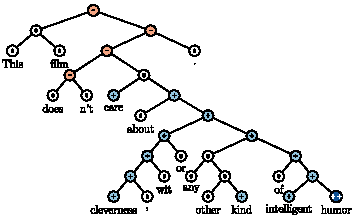
\includegraphics[width=0.6\linewidth]{./img/_sentiment_parse_tree.pdf}
                    \end{figure}
                    Due to the negation (\texttt{doesn't}), the whole positive sequence is negated.
                \end{example}
        \end{description}

    \item[Sentiment lexicon] \marginnote{Sentiment lexicon}
        If training data is insufficient, external domain knowledge, such as sentiment lexicon, can be used.

        \begin{example}
            A possible way to use a lexicon is to count the number of positive and negative words according to that corpus.
        \end{example}

        \begin{remark}
            Possible ways to create a lexicon are through:
            \begin{itemize}
                \item Expert annotators.
                \item Crowdsourcing in a two-step procedure:
                    \begin{enumerate}
                        \item Ask questions related to synonyms (e.g., which word is closest in meaning to \textit{startle}?).
                        \item Rate the association of words with emotions (e.g., how does \textit{startle} associate with \textit{joy}, \textit{fear}, \textit{anger}, \dots?).
                    \end{enumerate}
                \item Semi-supervised induction of labels from a small set of annotated data (i.e., seed labels). It works by looking for words that appear together with the ones with a known sentiment.
                \item Supervised learning using annotated data.
            \end{itemize}
        \end{remark}
\end{descriptionlist}


\subsection{Properties}

Naive Bayes has the following properties:
\begin{itemize}
    \item It is generally effective with short sequences and fewer data samples.
    \item It is robust to irrelevant features (i.e., words that appear in both negative and positive sentences) as they cancel out each other.
    \item It has good performance in domains with many equally important features (contrarily to decision trees).
    \item The independence assumption might produce overestimated predictions.
\end{itemize}

\begin{remark}
    Naive Bayes is a good baseline when experimenting with text classifications.
\end{remark}



\section{Logistic regression}

\begin{description}
    \item[Features engineering] \marginnote{Features engineering}
        Determine features by hand from the data (e.g., number of positive and negative lexicon).


    \item[Binary logistic regression] \marginnote{Binary logistic regression}
        Discriminative probabilistic model that computes the joint distribution $\prob{c | d}$ of the class $c$ given the document $d$.

        Given the input features $\vec{x} = [x_1, \dots, x_n]$, logistic regression computes the following:
        \[ 
            \sigma\left( \sum_{i=1}^{n} w_i x_i + b \right) = \sigma(\vec{w}\vec{x} + b)
        \]
        where $\sigma$ is the sigmoid function.

        \begin{description}
            \item[Loss]
                The loss function should aim to maximize the probability of predicting the correct label $\hat{y}$ given the observation $\vec{x}$. This can be expressed as a Bernoulli distribution:
                \[ 
                    \prob{y | x} = \hat{y}^y (1-\hat{y})^{1-y} = \begin{cases}
                        1 - \hat{y} & \text{if $y=0$} \\
                        \hat{y} & \text{if $y=1$} \\
                    \end{cases} 
                \]
                By applying a log-transformation and inverting the sign, this corresponds to the cross-entropy loss in the binary case:
                \[ \mathcal{L}_{\text{BCE}}(\hat{y}, y) = -\log \prob{y | x} = -[y \log(\hat{y}) + (1-y)\log(1-\hat{y})] \]

            \item[Optimization]
                As cross-entropy is convex, SGD is well suited to find the parameters $\vec{\theta}$ of a logistic regressor $f$ over batches of $m$ examples by solving:
                \[ \arg\min_{\vec{\theta}} \sum_{i=1}^{m} \mathcal{L}_\text{BCE}(\hat{y}^{(i)}, f(x^{(i)}; \vec{\theta})) + \alpha \mathcal{R}(\vec{\theta}) \]
                where $\alpha$ is the regularization factor and $\mathcal{R}(\vec{\theta})$ is the regularization term. Typical regularization approaches are:
                \begin{descriptionlist}
                    \item[Lasso regression (L1)] $\mathcal{R}(\vec{\theta}) = \Vert \vec{\theta} \Vert_1 = \sum_{j=1}^{n} \vert \vec{\theta}_j \vert$.
                    \item[Ridge regression (L2)] $\mathcal{R}(\vec{\theta}) = \Vert \vec{\theta} \Vert^2_2 = \sum_{j=1}^{n} \vec{\theta}_j^2$.
                \end{descriptionlist}
        \end{description}

    \item[Multinomial logistic regression] \marginnote{Multinomial logistic regression}
        Extension of logistic regression to the multi-class case. The joint probability becomes $\prob{y = c | x}$ and softmax is used in place of the sigmoid.

        Cross-entropy is extended over the classes $C$:
        \[ \mathcal{L}_\text{CE}(\hat{y}, y) = - \sum_{c \in C} \mathbbm{1}\{y = c\} \log(\prob{y = c | x}) \]
\end{description}


\subsection{Properties}

Logistic regression has the following properties:
\begin{itemize}
    \item It is generally effective with large documents or datasets.
    \item It is robust to correlated features.
\end{itemize}

\begin{remark}
    Logistic regression is also a good baseline when experimenting with text classifications.

    As they are lightweight to train, it is a good idea to test both naive Bayes and logistic regression to determine the best baseline for other experiments.
\end{remark}



\section{Metrics}


\subsection{Binary classification}

\begin{description}
    \item[Contingency table] \marginnote{Contingency table}
        $2 \times 2$ table matching predictions to ground truths. It contains true positives (\texttt{TP}), false positives (\texttt{FP}), false negatives (\texttt{FN}), and true negatives (\texttt{TN}).

    \item[Recall] \marginnote{Recall} 
        $\frac{\texttt{TP}}{\texttt{TP} + \texttt{FN}}$.

    \item[Precision] \marginnote{Precision} 
        $\frac{\texttt{TP}}{\texttt{TP} + \texttt{FP}}$.

    \item[Accuracy] \marginnote{Accuracy} 
        $\frac{\texttt{TP} + \texttt{TN}}{\texttt{TP} + \texttt{FP} + \texttt{FN} + \texttt{TN}}$.

        \begin{remark}
            Accuracy is a reasonable metric only when classes are balanced.
        \end{remark}

    \item[F1 score] \marginnote{F1 score} 
        $\frac{2 \cdot \texttt{recall} \cdot \texttt{precision}}{\texttt{recall} + \texttt{precision}}$.
\end{description}


\subsection{Multi-class classification}

\begin{description}
    \item[Confusion matrix] \marginnote{Confusion matrix}
        $c \times c$ table matching predictions to ground truths.

    \item[Precision/Recall] \marginnote{Precision/Recall}
        Precision and recall can be defined class-wise (i.e., consider a class as the positive label and the others as the negative).

    \item[Micro-average precision/recall] \marginnote{Micro-average precision/recall}
        Compute the contingency table of each class and collapse them into a single table. Compute precision or recall on the pooled contingency table.

        \begin{remark}
            This approach is sensitive to the most frequent class.
        \end{remark}

    \item[Macro-average precision/recall] \marginnote{Macro-average precision/recall}
        Compute precision or recall class-wise and then average over the classes.

        \begin{remark}
            This approach is reasonable if the classes are equally important.
        \end{remark}

        \begin{remark}
            Macro-average is more common in NLP.
        \end{remark}
\end{description}

\begin{example}
    \phantom{}

    \begin{figure}[H]
        \centering
        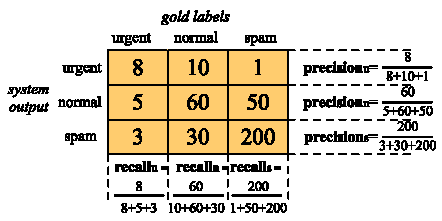
\includegraphics[width=0.5\linewidth]{./img/_confusion_matrix_example.pdf}
        \caption{Confusion matrix}
    \end{figure}

    \begin{figure}[H]
        \centering
        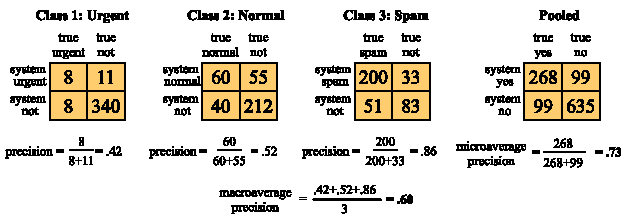
\includegraphics[width=0.85\linewidth]{./img/_micro_macro_average_example.pdf}
        \caption{
            \parbox[t]{0.6\linewidth}{
                Class-wise contingency tables, pooled contingency table, and micro/macro-average precision
            }
        }
    \end{figure}
\end{example}


\subsection{Cross-validation}

\begin{description}
    \item[$\mathbf{n}$-fold cross-validation] \marginnote{$n$-fold cross-validation}
        Tune a classifier on different sections of the training data:
        \begin{enumerate}
            \item Randomly choose a training and validation set.
            \item Train the classifier.
            \item Evaluate the classifier on a held-out test set.
            \item Repeat for $n$ times.
        \end{enumerate}
\end{description}

\subsection{Statistical significance}

\begin{description}
    \item[$\mathbf{p}$-value] \marginnote{$p$-value}
        Measure to determine whether a model $A$ is outperforming a model $B$ on a given test set by chance (i.e., test the null hypothesis $H_0$ or, in other words, test that there is no relation between $A$ and $B$).

        Given:
        \begin{itemize}
            \item A test set $x$,
            \item A random variable $X$ over the test sets (i.e., another test set),
            \item Two models $A$ and $B$, such that $A$ is better than $B$ by $\delta(x)$ on the test set $x$,
        \end{itemize}
        the $p$-value is defined as:
        \[ p\text{-value}(x) = \prob{\delta(X) > \delta(x) | H_0} \]
        There are two cases:
        \begin{itemize}
            \item $p\text{-value}(x)$ is big: the null hypothesis holds (i.e., $\prob{\delta(X) > \delta(x)}$ is high under the assumption that $A$ and $B$ are not related), so $A$ outperforms $B$ by chance.
            \item $p\text{-value}(x)$ is small (i.e., $< 0.05$ or $< 0.01$): the null hypothesis is rejected, so $A$ actually outperforms $B$.
        \end{itemize}

    \item[Bootstrapping test] \marginnote{Bootstrapping test}
        Approach to compute $p$-values.

        Given a test set $x$, multiple virtual test sets $\bar{x}^{(i)}$ are created by sampling with replacement (it is assumed that the new sets are representative). The performance difference $\delta(\cdot)$ is computed between two models and the $p$-value is determined as the frequency of:
        \[ \delta(\bar{x}^{(i)}) > 2\delta(x) \]

        \begin{remark}
            $\delta(x)$ is doubled due to theoretical reasons.
        \end{remark}

        \begin{example}
            Consider two models $A$ and $B$, and a test set $x$ with 10 samples. From $x$, multiple new sets (in this case of the same size) can be sampled. In the following table, each cell indicates which model correctly predicted the class:
            \begin{center}
                \footnotesize
                \begin{tabular}{ccccccccccc|ccc}
                    \toprule
                                    & 1 & 2 & 3 & 4 & 5 & 6 & 7 & 8 & 9 & 10 & $A\%$ & $B\%$ & $\delta(\cdot)$ \\
                    \midrule
                    $x$             & $AB$ & $A$ & $AB$ & $B$ & $A$ & $B$ & $A$ & $AB$ & -- & $A$ & $0.7$ & $0.5$ & $0.2$ \\
                    $\bar{x}^{(1)}$   & $A$ & $AB$ & $A$ & $B$ & $B$ & $A$ & $B$ & $AB$ & -- & $AB$ & $0.6$ & $0.6$ & $0.0$ \\
                    $\vdots$ & $\vdots$ & $\vdots$ & $\vdots$ & $\vdots$ & $\vdots$ & $\vdots$ & $\vdots$ & $\vdots$ & $\vdots$ & $\vdots$ & $\vdots$ & $\vdots$ & $\vdots$ \\
                    \bottomrule
                \end{tabular}
            \end{center}
            A possible way to sample $\bar{x}^{(1)}$ is (w.r.t. the indexes of the examples in $x$) $[2, 3, 3, 2, 4, 6, 2, 4, 1, 9, 1]$.
        \end{example}
\end{description}



\section{Affective meaning} \label{sec:affective_meaning}

The affective meaning of a text corpus can vary depending on:
\begin{descriptionlist}
    \item[Personality traits] 
        Stable behavior and personality of a person (e.g., nervous, anxious, reckless, \dots).

    \item[Attitude] 
        Enduring sentiment towards objects or people (e.g., liking, loving, hating, \dots).

    \item[Interpersonal stance] 
        Affective stance taken in a specific interaction (e.g., distant, cold, warm, \dots).

    \item[Mood] 
        Affective state of low intensity and long duration often without an apparent cause (e.g., cheerful, gloomy, irritable, \dots).

    \item[Emotion] 
        Brief response to an external or internal event of major significance (e.g., angry, sad, joyful, \dots).

        \begin{remark}
            Emotion is the most common subject in affective computing.
        \end{remark}
\end{descriptionlist}


\subsection{Emotion}

\begin{description}
    \item[Theory of emotion]
        There are two main theories of emotion:
        \begin{descriptionlist}
            \item[Basic emotions] \marginnote{Basic emotions}
                Discrete and fixed range of atomic emotions.

                \begin{remark}
                    Emotions associated to a word might be in contrast. For instance, in the NRC Word-Emotion Association Lexicon the word \texttt{thirst} is associated to both \textit{anticipation} and \textit{surprise}.
                \end{remark}

            \item[Continuum emotions] \marginnote{Continuum emotions}
                Describe emotions in a 2 or 3 dimensional space with the following features:
                \begin{descriptionlist}
                    \item[Valence] Pleasantness of a stimulus.
                    \item[Arousal] Intensity of emotion.
                    \item[Dominance] Degree of control on the stimulus.
                \end{descriptionlist}

                \begin{remark}
                    Valence is often used as a measure of sentiment.
                \end{remark}
        \end{descriptionlist}
\end{description}
    \chapter{Regression}

\begin{description}
    \item[Linear regression] \marginnote{Linear regression}
        Given:
        \begin{itemize}
            \item A dataset $\matr{X}$ of $N$ rows and $D$ features.
            \item A response vector $\vec{y}$ of $N$ continuous values.
        \end{itemize}
        We want to learn the parameters $\vec{w} \in \mathbb{R}^D$ such that:
        \[ \vec{y} \approx \matr{X}\vec{w}^T \]

    \item[Mean squared error] \marginnote{Mean squared error}
        To find the parameters for linear regression,
        we minimize as loss function the mean squared error:
        \[  
            \mathcal{L}(\vec{w}) = \Vert \matr{X}\vec{w}^T - \vec{y} \Vert^2    
        \]
        Its gradient is:
        \[ \nabla\mathcal{L}(\vec{w}) = 2\matr{X}^T(\matr{X}\vec{w}^T - \vec{y}) \]
        Constraining it to 0, we obtain the problem:
        \[ \matr{X}^T\matr{X}\vec{w}^T = \matr{X}^T\vec{y} \]
        If $\matr{X}^T\matr{X}$ is invertible, this can be solved analytically but could lead to overfitting.
        Numerical methods are therefore more suited.

        Note that:
        \begin{itemize}
            \item MSE is influenced by the magnitude of the data.
            \item It measures the fitness of a model in absolute terms.
            \item It is suited to compare different models.
        \end{itemize}

    \item[Coefficient of determination] \marginnote{Coefficient of determination}
        Given:
        \begin{itemize}
            \item The mean of the observed data: $y_\text{avg} = \frac{1}{N} \sum_i \vec{y}_i$.
            \item The sum of the squared residuals: $SS_\text{res} = \sum_i (\vec{y}_i - \vec{w}^T\vec{x}_i)^2$.
            \item The total sum of squares: $SS_\text{tot} = \sum_i (\vec{y}_i - y_\text{avg})^2$.
        \end{itemize}
        The coefficient of determination is given by:
        \[ \text{R}^2 = 1 - \frac{SS_\text{res}}{SS_\text{tot}} \]

        Intuitively, $\text{R}^2$ compares the model with a horizontal straight line ($y_\text{avg}$).
        When $\text{R}^2 = 1$, the model has a perfect fit.
        When $\text{R}^2$ is outside the range $[0, 1]$, then the model is worse than a straight line.

        Note that:
        \begin{itemize}
            \item $\text{R}^2$ is a standardized index.
            \item $\text{R}^2$ tells how well the variables of the predictor can explain the variation in the target.
            \item $\text{R}^2$ is not suited for non-linear models.
        \end{itemize}

    \item[Polynomial regression] \marginnote{Polynomial regression}
        Find a polynomial instead of a hyperplane.
\end{description}
    \chapter{Clustering}


\section{Similarity and dissimilarity}

\begin{description}
    \item[Similarity] \marginnote{Similarity}
        Measures how alike two objects are.
        Often defined in the range $[0, 1]$.

    \item[Dissimilarity] \marginnote{Dissimilarity}
        Measures how two objects differ.
        0 indicates no difference while the upper bound varies.
\end{description}

\begin{table}[ht]
    \centering
    \renewcommand{\arraystretch}{2}
    \begin{tabular}{c | c | c}
        \textbf{Attribute type} & \textbf{Dissimilarity} & \textbf{Similarity} \\
        \hline
        Nominal & $d(p, q) = \begin{cases} 0 & \text{if } p=q \\ 1 & \text{if } p \neq q \end{cases}$ & $s(p, q) = 1 - d(p, q)$ \\
        \hline
        Ordinal & $d(p, q) = \frac{\vert p - q \vert}{V}$ with $p, q \in \{ 0, \dots, V \}$ & $s(p, q) = 1 - d(p, q)$ \\
        \hline
        Interval or ratio & $d(p, q) = \vert p - q \vert$ & $s(p, q) = \frac{1}{1 + d(p, q)}$
    \end{tabular}
    \caption{Similarity and dissimilarity by attribute type}
\end{table}

\begin{description}
    \item[Similarity properties] \phantom{}
        \begin{enumerate}
            \item $\texttt{sim}(p, q) = 1$ iff $p = q$. 
            \item $\texttt{sim}(p, q) = \texttt{sim}(q, p)$. 
        \end{enumerate}
\end{description}


\subsection{Distance}

Given two $D$-dimensional data entries $p$ and $q$, possible distance metrics are:
\begin{descriptionlist}
    \item[Minkowski distance ($L_r$)] \marginnote{Minkowski distance}
        \[ \texttt{dist}(p, q) = \left( \sum_{d=1}^{D} \vert p_d - q_d \vert^r \right)^{\frac{1}{r}} \]
        where $r$ is a parameter.

        Common values for $r$ are:
        \begin{descriptionlist}
            \item[$r = 1$] 
                Corresponds to the $L_1$ norm.
                It is useful for discriminating 0 distance and near-0 distance as 
                an $\varepsilon$ change in the data corresponds to an $\varepsilon$ change in the distance.
            \item[$r = 2$]
                Corresponds to the Euclidean distance or $L_2$ norm.
            \item[$r = \infty$]
                Corresponds to the $L_\infty$ norm.
                Considers only the dimensions with the maximum difference.
        \end{descriptionlist}
    
    \item[Mahalanobis distance] \marginnote{Mahalanobis distance}
        \[ \texttt{dist}(p, q) = \sqrt{ (p-q) \matr{\Sigma}^{-1} (p-q)^T } \]
        where $\matr{\Sigma}$ is the covariance matrix of the dataset.
        The Mahalanobis distance of $p$ and $q$ increases when the segment connecting them 
        points towards a direction of greater variation of the data.

        \begin{figure}[h]
            \centering
            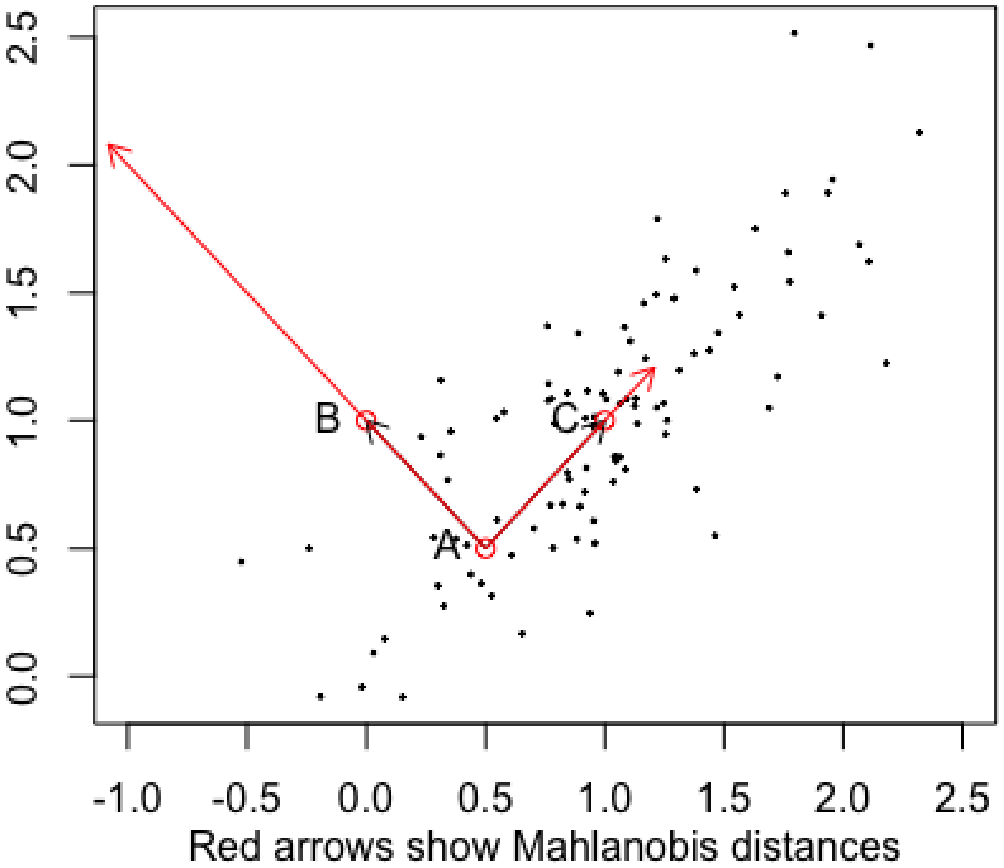
\includegraphics[width=0.35\textwidth]{img/mahalanobis.png}
            \caption{The Mahalanobis distance between $(A, B)$ is greater than $(A, C)$, while the Euclidean distance is the same.}
        \end{figure}
\end{descriptionlist}

\subsubsection{Distance properties}
\begin{descriptionlist}
    \item[Positive definiteness] 
        $\texttt{dist}(p, q) \geq 0$ and $\texttt{dist}(p, q) = 0$ iff $p = q$.
    \item[Symmetry] 
        $\texttt{dist}(p, q) = \texttt{dist}(q, p)$
    \item[Triangle inequality] 
        $\texttt{dist}(p, q) \leq \texttt{dist}(p, r) + \texttt{dist}(r, q)$
\end{descriptionlist}



\subsection{Vector similarity}

\begin{description}
    \item[Binary vectors]
        Given two examples $p$ and $q$ with binary features, we can compute the following values:
        \[ 
            \begin{split}
                M_{00} &= \text{ number of features that equals to 0 for both $p$ and $q$} \\
                M_{01} &= \text{ number of features that equals to 0 for $p$ and 1 for $q$} \\
                M_{10} &= \text{ number of features that equals to 1 for $p$ and 0 for $q$} \\
                M_{11} &= \text{ number of features that equals to 1 for both $p$ and $q$}
            \end{split}    
        \]
        Possible distance metrics are:
        \begin{descriptionlist}
            \item[Simple matching coefficient] \marginnote{Simple matching coefficient}
                $\texttt{SMC}(p, q) = \frac{M_{00} + M_{11}}{M_{00} + M_{01} + M_{10} + M_{11}}$ 
            \item[Jaccard coefficient] \marginnote{Jaccard coefficient}
                $\texttt{JC}(p, q) = \frac{M_{11}}{M_{01} + M_{10} + M_{11}}$ 
        \end{descriptionlist}

    \item[Cosine similarity] \marginnote{Cosine similarity}
        Cosine of the angle between two vectors:
        \[ \texttt{cos}(p, q) = \frac{p \cdot q}{\Vert p \Vert \cdot \Vert q \Vert} \]

    \item[Extended Jaccard coefficient (Tanimoto)] \marginnote{Extended Jaccard coefficient (Tanimoto)}
        Variation of the Jaccard coefficient for continuous values:
        \[ \texttt{T}(p, q) = \frac{p \cdot q}{\Vert p \Vert^2 + \Vert q \Vert^2 - p \cdot q} \]
\end{description}


\subsection{Correlation}

\begin{description}
    \item[Pearson's correlation] \marginnote{Pearson's correlation}
        Measure of linear relationship between a pair of quantitative attributes $e_1$ and $e_2$.
        To compute Pearson's correlation, the values of $e_1$ and $e_2$ are first standardized and then ordered to obtain the vectors $\vec{e}_1$ and $\vec{e}_2$.
        The correlation is then computed as the dot product between $\vec{e}_1$ and $\vec{e}_2$:
        \[ \texttt{corr}(e_1, e_2) = \langle \vec{e}_1, \vec{e}_2 \rangle \]

        Pearson's correlation has the following properties:
        \begin{itemize}
            \item If the variables are independent, then the correlation is 0 (but not vice versa).
            \item If the correlation is 0, then there is no linear relationship between the variables.
            \item $+1$ implies positive linear relationship, $-1$ implies negative linear relationship.
        \end{itemize}

    \item[Symmetric uncertainty] \marginnote{Symmetric uncertainty}
        Measure of correlation for nominal attributes:
        \[ U(e_1, e_2) = 2 \frac{H(e_1) + H(e_2) - H(e_1, e_2)}{H(e_1) + H(e_2)} \in [0, 1] \]
        where $H$ is the entropy.
\end{description}




\section{Clustering definitions}

\begin{description}
    \item[Clustering] \marginnote{Clustering}
        Given a set of $D$-dimensional objects $\vec{x}_i$, 
        we want to partition them into $K$ clusters (and potentially recognize outliers).
        In other words, we are looking for a mapping:
        \[ \texttt{cluster}(\vec{x}_i) \in \{ 1, \dots, K \} \]
        such that objects in the same cluster are similar.

    \item[Centroid] \marginnote{Centroid}
        Average of the coordinates of the points in a cluster.
        For a cluster $K_i$, the $d$-th coordinate of its centroid is given by:
        \[ 
            \texttt{centroid}(K_i)\texttt{[$d$]} 
                = \frac{1}{\vert K_i \vert} 
                    \sum_{\vec{x} \in K_i} \vec{x}\texttt{[$d$]} 
        \]

    \item[Medoid] \marginnote{Medoid}
        Element of the cluster with minimum average dissimilarity to all other points.
        Differently from the centroid, the medoid must be an existing point of the dataset.

    \item[Proximity functions] \marginnote{Proximity function} 
        Measures to determine the similarity of two data points:
        \begin{descriptionlist}
            \item[Euclidean distance] 
        \end{descriptionlist}
\end{description}


\section{Metrics}

\begin{description}
    \item[Cohesion] \marginnote{Cohesion}
        Measures the similarity (proximity) of the objects in the same cluster.
        Given a cluster $K_i$, cohesion is computed as:
        \[ \texttt{cohesion}(K_i) = \sum_{\vec{x} \in K_i} \texttt{dist}(\vec{x}, \vec{c}_i) \]
        where $\vec{c}_i$ can be the centroid or medoid
        and \texttt{dist} is a proximity function.

    \item[Separation] \marginnote{Separation}
        Measures the distance of two clusters.
        Given two clusters $K_i$ and $K_j$, their separation is:
        \[ \texttt{separation}(K_i, K_j) = \texttt{dist}(\vec{c}_i, \vec{c}_j) \]
        where $\vec{c}_i$ and $\vec{c}_j$ are respectively the centroids of $K_i$ and $K_j$, and \texttt{dist} is a proximity function.

    \item[Sum of squared errors] \marginnote{Sum of squared errors}
        Measures for each cluster the distance between its points to its centroid.
        Can be seen as the application of distortion (\Cref{desc:distortion}) to clustering:
        \[ \texttt{SSE}_j = \sum_{\vec{x}_i \in K_j} \texttt{dist}(\vec{x}_i, \vec{c}_j)^2 \]
        where $K_j$ is the $j$-th cluster and $\vec{c}_j$ is its centroid.

        If $\texttt{SSE}_j$ is high, the cluster has low quality.
        If $\texttt{SSE}_j = 0$, all points in the cluster correspond to the centroid.

        The sum of squared errors of $K$ clusters is:
        \[ \texttt{SSE} = \sum_{j=1}^{K} \texttt{SSE}_j \]

    \item[Sum of squares between clusters] \marginnote{Sum of squares between clusters}
        Given the global centroid of the dataset $\vec{c}$ and
        $K$ clusters each with $N_i$ objects,
        the sum of squares between clusters is given by:
        \[ \texttt{SSB} = \sum_{i=1}^{K} N_i \cdot \texttt{dist}(\vec{c}_i, \vec{c})^2 \]

    \item[Total sum of squares] \marginnote{Total sum of squares}
        Sum of the squared distances between the points of the dataset and the global centroid.
        It can be shown that the total sum of squares can be computed as:
        \[ \texttt{TSS} = \texttt{SSE} + \texttt{SSB} \]

        \begin{theorem}
            Minimize \texttt{SSE} $\iff$ maximize \texttt{SSB}.
        \end{theorem}
        
    \item[Silhouette score] \marginnote{Silhouette score}
        The Silhouette score of a data point $\vec{x}_i$ belonging to a cluster $K_i$ is given by two components:
        \begin{description}
            \item[Sparsity contribution] 
                The average distance of $\vec{x}_i$ to the other points in $K_i$:
                \[ a(\vec{x}_i) = \frac{1}{\vert K_i \vert - 1} \sum_{\vec{x}_j \in K_i, \vec{x}_j \neq \vec{x}_i} \texttt{dist}(\vec{x}_i, \vec{x}_j) \]
            
            \item[Separation contribution] 
                The average distance of $\vec{x}_i$ to the points in the nearest cluster:
                \[ b(\vec{x}_i) = \min_{K_j, K_j \neq K_i} \left( \frac{1}{\vert K_j \vert} \sum_{\vec{w} \in K_j} \texttt{dist}(\vec{x}_i, \vec{w}) \right) \]
        \end{description}
        The Silhouette score of $\vec{x}_i$ is then computed as:
        \[ s(\vec{x}_i) = \frac{b(\vec{x}_i) - a(\vec{x}_i)}{\max\{ a(\vec{x}_i), b(\vec{x}_i) \}} \in [-1, 1] \]
        
        The Silhouette score $\mathcal{S}$ of $K$ clusters is given by the average Silhouette scores of each data point.
        $\mathcal{S} \rightarrow 1$ indicates correct clusters, $\mathcal{S} \rightarrow -1$ indicates incorrect clusters.

    \item[Golden standard] \marginnote{Golden standard}
        Evaluation using a labeled dataset.
        Consider the elements of the same cluster as labeled with the same class.

        \begin{description}
            \item[Classification-oriented] 
                Traditional classification metrics such as accuracy, recall, precision, \dots

            \item[Similarity-oriented]
                Given a learnt clustering scheme $y_K(\cdot)$ and the golden standard scheme $y_G(\cdot)$ where 
                $y_i(\vec{x})$ indicates the label/cluster of $\vec{x}$, each pair of data $(\vec{x}_1, \vec{x}_2)$ can be labeled with:
                \begin{descriptionlist}
                    \item[\texttt{SGSK}] if $y_G(\vec{x}_1) = y_G(\vec{x}_2)$ and $y_K(\vec{x}_1) = y_K(\vec{x}_2)$.
                    \item[\texttt{SGDK}] if $y_G(\vec{x}_1) = y_G(\vec{x}_2)$ and $y_K(\vec{x}_1) \neq y_K(\vec{x}_2)$.
                    \item[\texttt{DGSK}] if $y_G(\vec{x}_1) \neq y_G(\vec{x}_2)$ and $y_K(\vec{x}_1) = y_K(\vec{x}_2)$.
                    \item[\texttt{DGDK}] if $y_G(\vec{x}_1) \neq y_G(\vec{x}_2)$ and $y_K(\vec{x}_1) \neq y_K(\vec{x}_2)$.
                \end{descriptionlist}
                Then, the following metrics can be computed:
                \begin{descriptionlist}
                    \item[Rand score] $\frac{\texttt{SGSK} + \texttt{DGDK}}{\texttt{SGSK} + \texttt{SGDK} + \texttt{DGSK} + \texttt{DGDK}}$
                    \item[Adjusted rand score] Modification of the rand score to take into account that some agreements may happen by chance.
                    \item[Jaccard coefficient] For each class $c$, the Jaccard coefficient is given by:
                        \[ \frac{\texttt{SG$_c$SK$_c$}}{\texttt{SG$_c$SK$_c$} + \texttt{SG$_c$DK$_c$} + \texttt{DG$_c$SK$_c$}} \]
                \end{descriptionlist}
        \end{description}
\end{description}



\section{K-means}

\begin{description}
    \item[Algorithm] \marginnote{K-means}
        Clustering algorithm that iteratively improves the centroids.
        Given the desired number of clusters $K$, the algorithm works as follows:
        \begin{enumerate}
            \item Randomly choose $K$ initial centroids.
            \item Each data point belongs to the cluster represented by the nearest centroid.
            \item Update the centroids as the centroids of the newly found clusters. Go to 2.
        \end{enumerate}

    \item[Distortion] \label{desc:distortion} \marginnote{Distortion}
        Given:
        \begin{itemize}
            \item a $D$-dimensional dataset of $N$ points $\vec{x}_i$;
            \item an encoding function $\texttt{encode}: \mathbb{R}^D \rightarrow [1, K]$;
            \item a decoding function $\texttt{decode}: [1, K] \rightarrow \mathbb{R}^D$.
        \end{itemize}
        Distortion (or inertia) is defined as:
        \[ \texttt{distortion} = \sum_{i=1}^{N} \big(\vec{x}_i - \texttt{decode}(\texttt{encode}(\vec{x_i})) \big)^2 \]

        \begin{theorem}
            To minimize the distortion, it is required that:
            \begin{enumerate}
                \item $\vec{x}_i$ is encoded with its nearest center.
                \item The center of a point is the centroid of the cluster it belongs to.
            \end{enumerate}

            Note that k-means alternates points 1 and 2.

            \begin{proof}
                The second point is derived by imposing the derivative of \texttt{distortion} to 0.
            \end{proof}
        \end{theorem}

    \item[Elbow method]
        Inertia decreases monotonically and can be used to determine an ideal number of clusters.
        By computing the inertia for varying $K$, a plausible value is the one corresponding to the point where the slope decreases.
        \begin{figure}[H]
            \centering
            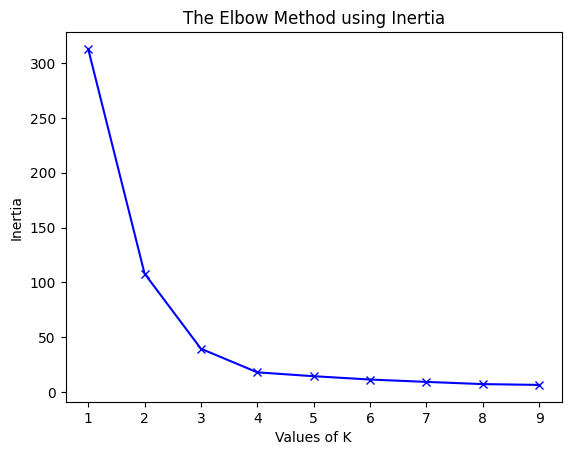
\includegraphics[width=0.4\textwidth]{img/elbow_method.png}
            \caption{Plot of inertia. Possibly good values for $K$ are around 3}
        \end{figure}

        The Silhouette score can also be used by selecting the $K$ corresponding to its maximum.
        Note that, compared to inertia, Silhouette is computationally more expensive.

    \item[Properties] \phantom{}
        \begin{description}
            \item[Termination] 
                There are a finite number of ways to cluster $N$ objects into $K$ clusters.
                By construction, at each iteration, the \texttt{distortion} is reduced.
                Therefore, k-means is guaranteed to terminate.

            \item[Non-optimality] 
                The solution found by k-means is not guaranteed to be a global best.
                The choice of starting points heavily influences the final result. 
                The starting configuration is usually composed of points distant as far as possible.

            \item[Noise]
                Outliers heavily influence the clustering result. Sometimes, it is useful to remove them.

            \item[Complexity]
                Given a $D$-dimensional dataset of $N$ points,
                running k-means for $T$ iterations to find $K$ clusters has complexity $O(TKND)$.
        \end{description}
\end{description}



\section{Hierarchical clustering}

\begin{description}
    \item[Dendrogram] \marginnote{Dendrogram}
        Tree-like structure where the root is a cluster of all the data points and 
        the leaves are clusters with a single data point.

    \item[Agglomerative] \marginnote{Agglomerative} 
        Starts with a cluster per data point and iteratively merges them (leaves to root).
        Uses cluster separation metrics.

    \item[Divisive] \marginnote{Divisive} 
        Starts with a cluster containing all the data points and iteratively splits them (root to leaves).
        Uses cluster cohesion metrics.

    \item[Cluster separation measures]
        Measure the distance between two clusters $K_i$ and $K_j$.
        \begin{descriptionlist}
            \item[Single link] \marginnote{Single link}
                Minimum distance of the points in the two clusters:
                \[ \texttt{sep}(K_i, K_j) = \min_{\vec{x} \in K_i, \vec{y} \in K_j} \texttt{dist}(\vec{x}, \vec{y}) \]
                Tends to create larger clusters.
    
            \item[Complete link] \marginnote{Complete link}
                Maximum distance of the points in the two clusters:
                \[ \texttt{sep}(K_i, K_j) = \max_{\vec{x} \in K_i, \vec{y} \in K_j} \texttt{dist}(\vec{x}, \vec{y}) \]
                Tends to create more compact clusters.
        
            \item[Average link] \marginnote{Average link}
                Average distance of the points in the two clusters:
                \[ \texttt{sep}(K_i, K_j) = \frac{1}{\vert K_i \vert \cdot \vert K_j \vert} \sum_{\vec{x} \in K_i, \vec{y} \in K_j} \texttt{dist}(\vec{x}, \vec{y}) \]
            
            \item[Centroid-based] \marginnote{Centroid-based}
                Distance between the centroids of the two clusters.

            \item[Ward's method] \marginnote{Ward's method}
                Let $K_m$ be the cluster obtained by merging $K_i$ and $K_j$.
                The distance between $K_i$ and $K_j$ is determined as:
                \[ \texttt{sep}(K_i, K_j) = \texttt{SSE}(K_m) - \big( \texttt{SSE}(K_i) + \texttt{SSE}(K_j) \big) \]
        \end{descriptionlist}
\end{description}


\subsection{Agglomerative clustering}

\begin{description}
    \item[Algorithm] \marginnote{Agglomerative clustering} \phantom{}
        \begin{enumerate}
            \item Initialize a cluster for each data point.
            \item Compute the distance matrix between each cluster.
            \item Merge the two clusters with the lowest separation, 
                drop their values from the distance matrix and add a row/column for the newly created cluster.
            \item Go to point 2. if the number of clusters is greater than one.
        \end{enumerate}

        After the construction of the dendrogram, a cut \marginnote{Cut} can be performed at a user-defined level.
        A cut near the root will result in few bigger clusters.
        A cut near the leaves will result in numerous smaller clusters.
        

    \item[Properties] \phantom{}
        \begin{description}
            \item[Complexity] 
                Space complexity of $O(N^2)$ to store the distance matrix.
                
                Time complexity of $O(N^3)$ ($O(N)$ iterations with a $O(N^2)$ search for the pair to merge and $O(N)$ to recompute the distance matrix) 
                that can be reduced to $O(N^2\log(N))$ when using indexing.
        \end{description}
\end{description}



\section{Density-based clustering}

Consider as clusters the high-density areas of the data space.

\begin{description}
    \item[Grid-based] 
        Split the data space into a grid and count the number of points in each tile.

    \item[Object-centered] 
        Count, for each point, the number of neighbors within a radius.
\end{description}


\subsection{DBSCAN}

\begin{description}
    \item[Neighborhood] \marginnote{Neighborhood}
        Given a radius $\varepsilon$, the neighborhood of a point $\vec{x}$ are the points within an $\varepsilon$-sphere centered on $\vec{x}$.

    \item[Core point] \marginnote{Core point}
        Given a minimum number of neighbors $m$, 
        a point $\vec{x}$ is a core point if it has at least $m$ neighbors.

    \item[Border point] \marginnote{Border point}
        A point $\vec{x}$ is a border point if it is not a core point.

    \item[Directly density reachable] \marginnote{Directly density reachable}
        A point $\vec{p}$ is directly density reachable from $\vec{q}$ iff:
        \begin{itemize}
            \item $\vec{q}$ is a core point.
            \item $\vec{q}$ is a neighbor of $\vec{p}$.
        \end{itemize}

    \item[Density reachable] \marginnote{Density reachable}
        A point $\vec{p}$ is density reachable from $\vec{q}$ iff:
        \begin{itemize}
            \item $\vec{q}$ is a core point.
            \item There exists a sequence of points $\vec{s}_1, \dots, \vec{s}_z$ such that:
            \begin{itemize}
                \item $\vec{s}_1$ is directly density reachable from $\vec{q}$.
                \item $\vec{s}_{i+1}$ is directly density reachable from $\vec{s}_i$.
                \item $\vec{p}$ is directly density reachable from $\vec{s}_z$.
            \end{itemize}
        \end{itemize}

    \item[Density connected] \marginnote{Density connected}
        A point $\vec{p}$ is density connected to $\vec{q}$ iff there exists a point $\vec{s}$ 
        such that both $\vec{p}$ and $\vec{q}$ are density reachable from $\vec{s}$.

    \item[Algorithm] \marginnote{DBSCAN}
        Determine clusters as maximal sets of density connected points.
        Border points not density connected to any core point are labeled as noise.

        In other words, what happens is the following:
        \begin{itemize}
            \item Neighboring core points are part of the same cluster.
            \item Border points are part of the cluster of their nearest core point neighbor.
            \item Border points without a core point neighbor are noise.
        \end{itemize}

    \item[Properties] \phantom{}
        \begin{description}
            \item[Robustness]
                Able to find clusters of any shape and detect noise.

            \item[Hyperparameters]
                Sensible to the choice of the radius $\varepsilon$ and minimum neighbors $m$.

                \begin{description}
                    \item[K-distance method] \phantom{}
                        \begin{enumerate}
                            \item Determine for each point its $k$-distance as the distance to its $k$-nearest neighbors.
                            \item Sort the points by decreasing $k$-distance and plot them.
                            \item Use as possible $\varepsilon$ the values around the area where the slope decreases (similarly to the elbow method).
                        \end{enumerate}
                \end{description}

            \item[Complexity]
                Complexity of $O(N^2)$, reduced to $O(N \log N)$ if using spatial indexing.
        \end{description}
\end{description}


\subsection{DENCLUE}

\begin{description}
    \item[Kernel density estimation] \marginnote{Kernel density estimation}
        Statistical method to estimate the distribution of a dataset through a function.

        \begin{description}
            \item[Kernel function] \marginnote{Kernel function}
                Symmetric and monotonically decreasing function to describe the influence of a data point on its neighbors.

                A typical kernel function is the Gaussian.

            \item[Overall density function]
                The overall density of the dataset is obtained as the sum of the kernel function evaluated at each data point.

                \begin{figure}[H]
                    \centering
                    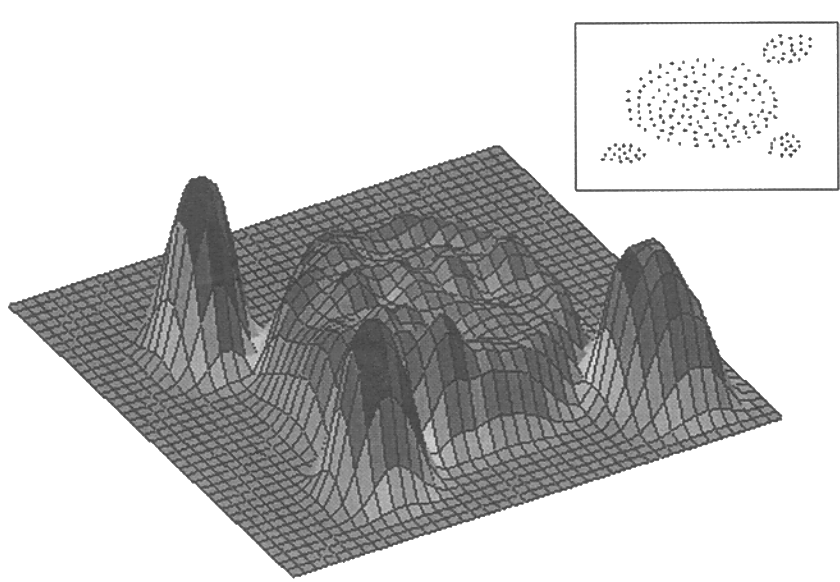
\includegraphics[width=0.35\textwidth]{img/kernel_density_estimation.png}
                    \caption{Example of density function from a set of points (top right) using a Gaussian kernel}
                    \label{img:denclue}
                \end{figure}
        \end{description}

    \item[Algorithm] \marginnote{DENCLUE}
        Given a threshold $\xi$, DENCLUE works as follows:
        \begin{enumerate}
            \item Derive a density function of the dataset.
            \item Identify local maximums and consider them as density attractors.
            \item Associate to each data point the density attractor in the direction of maximum increase.
            \item Points associated with the same density attractor are part of the same cluster.
            \item Remove clusters with a density attractor lower than $\xi$.
            \item Merge clusters connected through a path of points whose density is greater or equal to $\xi$ 
                (e.g. in \Cref{img:denclue} the center area will result in many small clusters that can be merged with an appropriate $\xi$).
        \end{enumerate}

    \item[Properties] \phantom{}
        \begin{description}
            \item[Robustness]
                Able to recognize clusters of different shapes and handle noise.

            \item[High dimension weakness]
                Does not perform well with high-dimensional data with different densities.

            \item[Complexity]
                Computational complexity of $O(N^2)$.
        \end{description}
\end{description}



\section{Model-based clustering}

Assuming that the attributes are independent random variables,
model-based clustering finds a set of distributions (one per cluster) that describe the data.


\subsection*{Gaussian mixture (expectation maximization)}

\begin{description}
    \item[Algorithm] \phantom{} \marginnote{Gaussian mixture} 
    \begin{enumerate}
        \item Select an initial set of parameters for the distributions.
        \item Expectation step: for each data point, compute its probability to belong to each distribution.
        \item Maximization step: tweak the parameters to maximize the likelihood (i.e. move the Gaussian towards the center of the cluster).
        \item Go to point 2. until convergence.
    \end{enumerate}
\end{description}
    \chapter{Association rules}


\section{Frequent itemset}

\begin{description}
    \item[Itemset] \marginnote{Itemset}
        Collection of one or more items (e.g. $\{ \text{milk}, \text{bread}, \text{diapers} \}$).

    \item[K-itemset] \marginnote{K-itemset}
        Itemset with $k$ items.

    \item[Support count] \marginnote{Support count}
        Number of occurrences of an itemset in a dataset.
        \begin{example}
            \phantom{}\\
            \begin{minipage}{0.4\textwidth}
                Given the following transactions:
                \begin{center}
                    \begin{tabular}{|c|l|}
                        \hline
                        1 & bread, milk \\
                        2 & beer, bread, diaper, eggs \\
                        3 & beer, coke, diaper, milk \\
                        \textbf{4} & \textbf{beer, bread, diaper, milk} \\
                        \textbf{5} & \textbf{bread, coke, diaper, milk} \\
                        \hline
                    \end{tabular}
                \end{center}
            \end{minipage}
            \begin{minipage}{0.5\textwidth}
                The support count of the itemset containing bread, diapers and milk is:
                \[ \sigma(\{ \text{bread}, \text{diapers}, \text{milk} \}) = 2 \]
            \end{minipage}
        \end{example}

        \item[Association rule] \marginnote{Association rule}
        Given two itemsets $A$ and $C$, an association rule has form:
        \[ A \rightarrow C \]
        It means that there are transactions in the dataset where $A$ and $C$ co-occur. 
        Note that it is not strictly a logical implication.

    \item[Metrics] \phantom{}
        \begin{description}
            \item[Support] \marginnote{Support}
            Given $N$ transactions, the support of an itemset $A$ is:
            \[ \texttt{sup}(A) = \frac{\sigma(A)}{N} \]
            The support of an association rule $A \rightarrow C$ is:
            \[ \texttt{sup}(A \rightarrow C) = \texttt{sup}(A \cup C) = \frac{\sigma(A \cup C)}{N} \]

            Low support implies random associations.

            \begin{description}
                \item[Frequent itemset] \marginnote{Frequent itemset}
                    Itemset whose support is at least a given threshold.
            \end{description}
    
        \item[Confidence] \marginnote{Confidence}
            Given an association rule $A \rightarrow C$, its confidence is given by:
            \[ \texttt{conf}(A \rightarrow C) = \frac{\sigma(A \cup C)}{\sigma(A)} \in [0, 1] \]

            Low confidence implies low reliability.

            \begin{theorem}
                The confidence of $A \rightarrow C$ can be computed given the supports of $A \rightarrow C$ and $A$:
                \[ \texttt{conf}(A \rightarrow C) = \frac{\texttt{sup}(A \rightarrow C)}{\texttt{sup}(A)} \]
            \end{theorem}
    \end{description}

    \item[Association rule mining] \marginnote{Association rule mining}
        Given $N$ transactions and two thresholds \texttt{min\_sup} and \texttt{min\_conf},
        association rule mining finds all the rules $A \rightarrow C$ such that:
        \[ \begin{split}
            \texttt{sup}(A \rightarrow C) &\geq \texttt{min\_sup} \\
            \texttt{conf}(A \rightarrow C) &\geq \texttt{min\_conf}
        \end{split} \]

        This can be done in two steps:
        \begin{enumerate}
            \item \marginnote{Frequent itemset generation}
                Determine the itemsets with $\text{support} \geq \texttt{min\_sup}$ (frequent itemsets).
            \item \marginnote{Rule generation}
                Determine the association rules with $\text{confidence} \geq \texttt{min\_conf}$.
        \end{enumerate}
\end{description}



\section{Frequent itemset generation}

\subsection{Brute force}
Given $D$ items, there are $2^D$ possible itemsets.
To compute the support of a single itemset, the complexity is $O(NW)$ where 
$N$ is the number of transactions and $W$ is the width of the largest transaction.
Listing all the itemsets and computing their support have an exponential complexity of $O(NW2^D)$.


\subsection{Apriori principle}

\begin{theorem} \marginnote{Apriori principle}
    If an itemset is frequent, then all of its subsets are frequent.

    \begin{proof}
        By the definition of support, it holds that:
        \[ \forall X, Y: (X \subseteq Y) \Rightarrow (\texttt{sup}(X) \geq \texttt{sup}(Y)) \]

        In other words, the support metric is anti-monotone.
    \end{proof}
\end{theorem}

\begin{corollary}
    If an itemset is infrequent, then all of its supersets are infrequent.
\end{corollary}

\begin{example} \phantom{}
    \begin{center}
        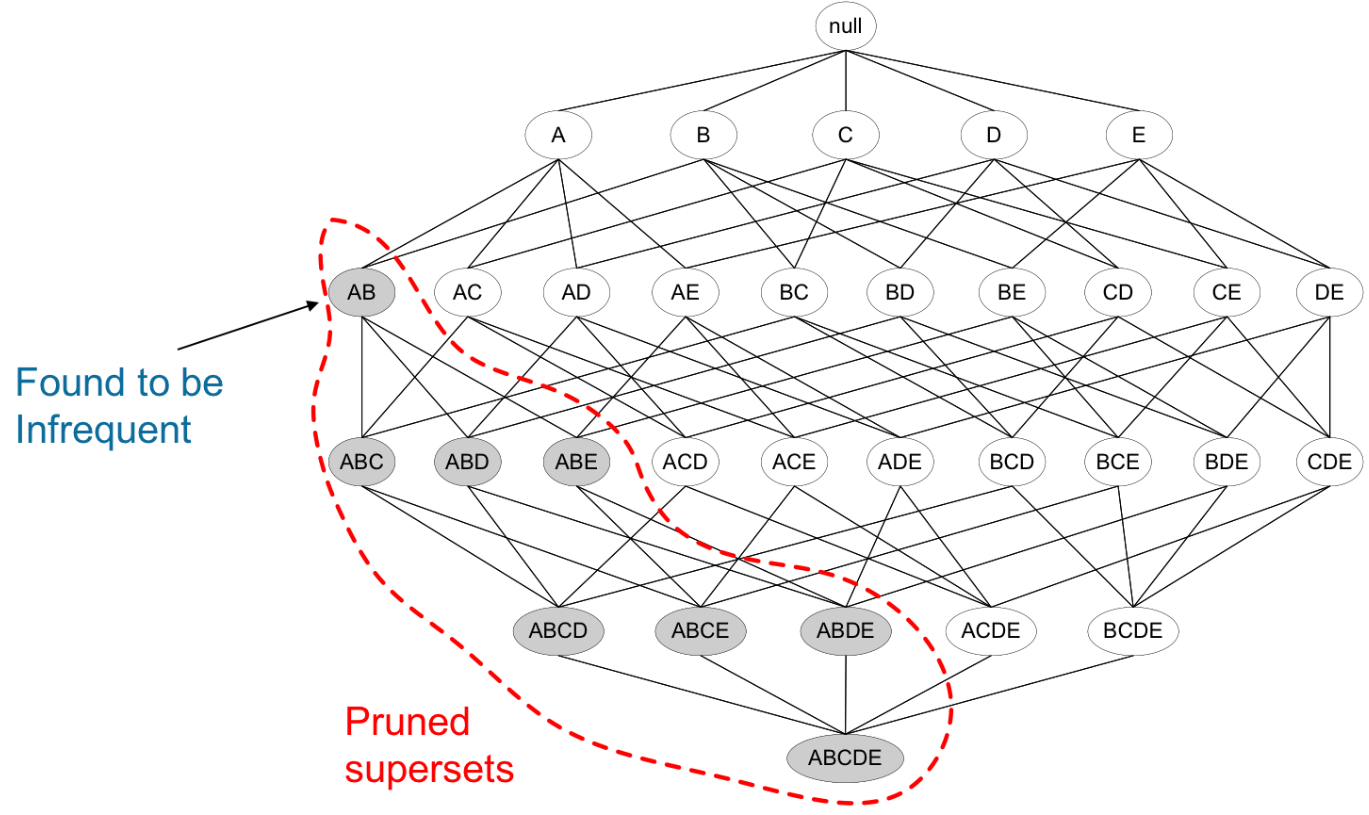
\includegraphics[width=0.6\textwidth]{img/itemset_apriori.png}
    \end{center}
\end{example}

\begin{algorithm}[H]
\caption{Apriori principle}
\begin{lstlisting}[mathescape=true]
def candidatesGeneration(freq_itemsets$_k$):
    candidate_itemsets$_{k+1}$ = selfJoin(freq_itemsets$_k$)
    for itemset in candidate_itemsets$_{k+1}$:
        for sub in subsetsOfSize($k$, itemset):
            if sub not in freq_itemsets$_k$:
                candidate_itemsets$_{k+1}$.remove(itemset)
    return candidate_itemsets$_{k+1}$

def aprioriItemsetGeneration(transactions, min_sup):
    freq_itemsets$_1$ = itemsetsOfSize(1, transactions)
    k = 1
    while freq_itemsets$_1$ is not null:
        candidate_itemsets$_{k+1}$ = candidatesGeneration(freq_itemsets$_k$)
        freq_itemsets$_{k+1}$ = $\{ c \in \texttt{candidate\_itemsets}_{k+1} \mid \texttt{sup(}c\texttt{)} \geq \texttt{min\_sup} \}$
        k += 1
    return freq_itemsets$_k$
\end{lstlisting}
\end{algorithm}

\begin{description}
    \item[Complexity]
        The complexity of the apriori principle depends on:
        \begin{itemize}
            \item The choice of the support threshold.
            \item The number of unique items.
            \item The number and the width of the transactions.
        \end{itemize}
\end{description}



\section{Rule generation}

\subsection{Brute force}
Given a frequent $k$-itemset $L$, there are $2^k-2$ possible association rules ($-2$ as $L \rightarrow \varnothing$ and $\varnothing \rightarrow L$ can be ignored).
For each possible rule, it is necessary to compute the confidence. The overall complexity is exponential.

\subsection{Apriori principle}

\begin{theorem} \marginnote{Apriori principle}
    Without loss of generality, consider an itemset $\{ A, B, C, D \}$.
    It holds that:
    \[ \texttt{conf}(ABC \rightarrow D) \geq \texttt{conf}(AB \rightarrow CD) \geq \texttt{conf}(A \rightarrow BCD) \]
\end{theorem}

\begin{example} \phantom{}
    \begin{center}
        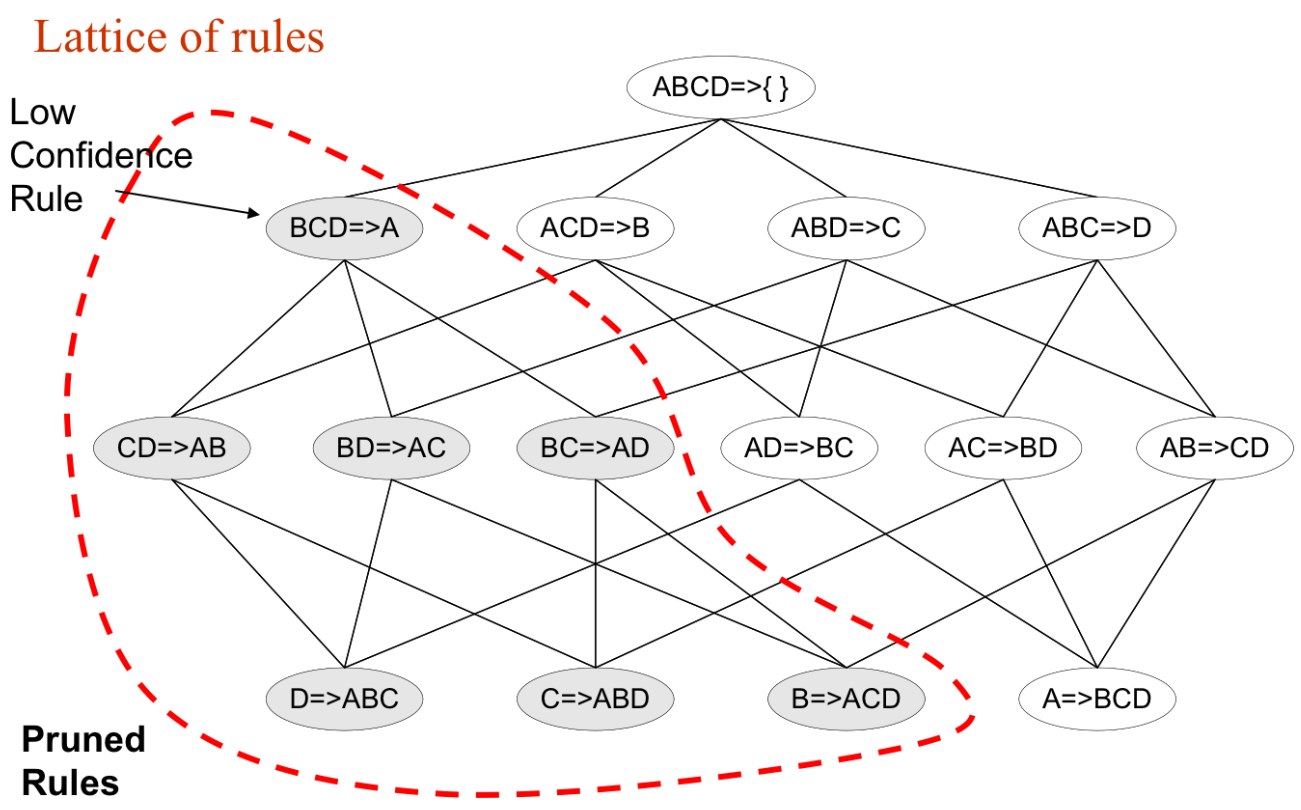
\includegraphics[width=0.5\textwidth]{img/rules_apriori.png}
    \end{center}
\end{example}



\section{Interestingness measures}

\begin{description}
    \item[Contingency table] \marginnote{Contingency table}
        Given an association rule $A \rightarrow C$, its contingency table is defined as:
        \begin{center}
            \def\arraystretch{1.1}
            \begin{tabular}{c|c|c|c}
                & $C$ & $\overline{C}$ & \\
                \hline
                $A$ & $\prob{A \land C}$ & $\prob{A \land \overline{C}}$ & $\prob{A}$ \\
                \hline
                $\overline{A}$ & $\prob{\overline{A} \land C}$ & $\prob{\overline{A} \land \overline{C}}$ & $\prob{\overline{A}}$ \\
                \hline
                & $\prob{C}$ & $\prob{\overline{C}}$ & 100 \\
            \end{tabular}
        \end{center}
\end{description}

\begin{remark}
    Confidence can be misleading.
    \begin{example} \phantom{}\\
        \begin{minipage}[t]{0.36\textwidth}
            Given the following contingency table:
            \begin{center}
                \begin{tabular}{c|c|c|c}
                                                & coffee    & $\overline{\text{coffee}}$ & \\
                    \hline
                    tea                         & 15        & 5                     & 20 \\
                    \hline
                    $\overline{\text{tea}}$     & 75        & 5                     & 80 \\
                    \hline
                                                & 90        & 10                    & 100 \\
                \end{tabular}
            \end{center}
        \end{minipage}
        \hspace{0.5cm}
        \begin{minipage}[t]{0.6\textwidth}
            We have that:
            \[ \texttt{conf}(\text{tea} \rightarrow \text{coffee}) = \frac{\texttt{sup}(\text{tea}, \text{coffee})}{\texttt{sup}(\text{tea})} = \frac{15}{20} = 0.75 \]
            But, we also have that:
            \[ \prob{\text{coffee}} = 0.9 \hspace*{1cm} \prob{\text{coffee} \mid \overline{\text{tea}}} = \frac{75}{80} = 0.9375 \]
            So, despite the high confidence of $(\text{tea} \rightarrow \text{coffee})$,
            the probability of coffee increases in absence of tea.
        \end{minipage}
    \end{example}
\end{remark}


\subsection{Statistical-based measures}

Measures that take into account the statistical independence of the items.

\begin{description}
    \item[Lift] \marginnote{Lift}
        \[ \texttt{lift}(A \rightarrow C) = \frac{\texttt{conf}(A \rightarrow C)}{\texttt{sup}(C)} = \frac{\prob{A \land C}}{\prob{A}\prob{C}} \]

        If $\texttt{lift}(A \rightarrow C) = 1$, then $A$ and $C$ are independent.
    
    \item[Leverage] \marginnote{Leverage}
        \[ \texttt{leve}(A \rightarrow C) = \texttt{sup}(A \cup C) - \texttt{sup}(A)\texttt{sup}(C) = \prob{A \land C} - \prob{A}\prob{C} \]
        
        If $\texttt{leve}(A \rightarrow C) = 0$, then $A$ and $C$ are independent.
    
    \item[Conviction] \marginnote{Conviction}
        \[ \texttt{conv}(A \rightarrow C) = \frac{1 - \texttt{sup}(C)}{1 - \texttt{conf}(A \rightarrow C)} = \frac{\prob{A}(1-\prob{C})}{\prob{A}-\prob{A \land C}} \]
\end{description}

\begin{table}[H]
    \centering
    \begin{tabular}{c|p{10cm}}
        \hline
        \textbf{Metric} & \textbf{Interpretation} \\
        \hline
        High support        & The rule applies to many transactions. \\
        \hline
        High confidence     & The chance that the rule is true for some transactions is high. \\
        \hline
        High lift           & Low chance that the rule is just a coincidence. \\
        \hline
        High conviction     & The rule is violated less often compared to the case when the antecedent and consequent are independent. \\
        \hline
    \end{tabular}
    \caption{Intuitive interpretation of the measures}
\end{table}



\section{Multi-dimensional association rules}

\begin{description}
    \item[Mono-dimensional events] \marginnote{Mono-dimensional events}
        Represented as transactions. Each event contains items that appear together.
        
    \item[Multi-dimensional events] \marginnote{Multi-dimensional events}
        Represented as tuples. Each event contains the values of its attributes.

    \item[Mono/Multi-dimensional equivalence] \marginnote{Equivalence}
        Mono-dimensional events can be converted into multi-dimensional events and vice versa.

        To transform quantitative attributes, it is usually useful to discretize them.

        \begin{example}[Multi to mono] \phantom{}\\
            \begin{minipage}{0.35\textwidth}
                \begin{center}
                    \begin{tabular}{c|c|c}
                        \textbf{Id} & \textbf{co2} & \textbf{tin\_oxide} \\
                        \hline
                        1 & high & medium \\
                        2 & medium & low \\
                    \end{tabular}
                \end{center}
            \end{minipage}
            $\rightarrow$
            \begin{minipage}{0.48\textwidth}
                \begin{center}
                    \begin{tabular}{c|c}
                        \textbf{Id} & \textbf{Transaction} \\
                        \hline
                        1 & $\{ \text{co2/high}, \text{tin\_oxide/medium} \}$ \\
                        2 & $\{ \text{co2/medium}, \text{tin\_oxide/low} \}$ \\
                    \end{tabular}
                \end{center}
            \end{minipage}
        \end{example}

        \begin{example}[Mono to multi] \phantom{}\\
            \begin{minipage}{0.35\textwidth}
                \begin{center}
                    \begin{tabular}{c|c|c|c|c}
                        \textbf{Id} & \textbf{a} & \textbf{b} & \textbf{c} & \textbf{d} \\
                        \hline
                        1 & yes & yes & no & no \\
                        2 & yes & no & yes & no \\
                    \end{tabular}
                \end{center}
            \end{minipage}
            $\leftarrow$
            \begin{minipage}{0.30\textwidth}
                \begin{center}
                    \begin{tabular}{c|c}
                        \textbf{Id} & \textbf{Transaction} \\
                        \hline
                        1 & $\{ \text{a}, \text{b} \}$ \\
                        2 & $\{ \text{a}, \text{c} \}$ \\
                    \end{tabular}
                \end{center}
            \end{minipage}
        \end{example}

\end{description}



\section{Multi-level association rules}
Organize items into a hierarchy.

\begin{description}
    \item[Specialized to general] \marginnote{Specialized to general} 
        Generally, the support of the rule increases.
        \begin{example}
            From $(\text{apple} \rightarrow \text{milk})$ to $(\text{fruit} \rightarrow \text{dairy})$
        \end{example}

    \item[General to specialized] \marginnote{General to specialized} 
        Generally, the support of the rule decreases.
        \begin{example}
            From $(\text{fruit} \rightarrow \text{dairy})$ to $(\text{apple} \rightarrow \text{milk})$
        \end{example}

    \item[Redundant level] \marginnote{Redundant level}
        A more specialized rule in the hierarchy is redundant if its confidence is similar to the one of a more general rule.

    \item[Multi-level association rule mining] \marginnote{Multi-level association rule mining}
        Run association rule mining on different levels of abstraction (general to specialized).
        At each level, the support threshold is decreased.
\end{description}

    \eoc

\end{document}